% Chapter Template

\chapter{Optogenetic Inactivation of Mouse Visual Area AM} % Main chapter title
\label{Chapter4} 

The results of the previous chapter demonstrated that mouse cortex, namely the posterior parietal cortex, was necessary for accurate performance on the visual pulses task. However, the findings, which result from inactivation of inhibitory neurons, are not straightforward to interpret. Suppressing the activity of inhibitory neurons, in principle, results in increased excitation within the area that then alters the amount of activity that downstream brain areas experience. However the effect may also be restricted locally and may not recapitulate the neural activity resulting from exogenous drive approaches like those previously used to disrupt behavior in rodents \parencite{Otchy2015,Rodgers2014,Licata2017}.\par 

As discussed in the Introduction (Chapter \ref{Chapter1}), the definition of mouse PPC and it's location relative to retinotopic extrastriate visual areas is not firmly established. Previous studies that investigated mouse PPC \parencite{Harvey2012,Marcos2016,Funamizu2016,Goard2016,Jeong2017} do not report the boundary extent of mouse PPC (defined by stereotactic coordinates). Furthermore, while \textcite{Funamizu2016} referred to mouse PPC as the area anterior to visual area PM, most studies did not reconcile the location of mouse PPC with respect to known mouse secondary visual area. \par

In humans and primates, PPC is located in between the somatosensory and the visual cortex. In the mouse brain, this location is occupied by several retinotopic extrastriate visual areas \parencite{Wang2007,Zhuang2017}. The anatomical position and distinct projection targets of visual areas located between V1 and S1 (namely areas A, AM, RL,MMA, and RLL) open up the possibility that one or several of these retinotopic extrastriate visual areas may possess functional properties analogous with visual parietal areas previously annotated with in nonhuman primates \parencite{Cavada1993}. Because the boundary extent of stereotactic mouse PPC \parencite{Harvey2012} is undefined, it not obvious whether this area overlaps with one or more retinotopic visual areas. \par 

A promising candidate for mouse PPC, or subdivision thereof, is visual area AM. Area AM has prominent projection patterns to frontal and motor areas, which resemble those observed in primate LIP (Table \ref{table:areaLIP}), and is therefore, in a position to play a key role in conveying visual information into motor output. Few studies have examined how visual areas beyond V1 contribute to sensory driven behavior in mouse. Furthermore, the perceptual decision making field has not taken full advantage of the tools available in mouse for causally linking neural activity to behavior, namely, careful anatomical distinction of extrastriate areas combined with functional manipulations. These efforts present an opportunity to ascertain whether visual areas in the mouse show functional similarities to areas already defined in non-human primate.\par 

Towards this goal, the experiments in this chapter test the causal role of visual area AM (a proposed subdivision of mouse PPC ) in evidence accumulation for visually-guided behavior. Furthermore, the experiments aim towards the ultimate goal of establishing behavioral consequences for, otherwise largely unknown roles of, mouse extrastriate visual areas during behavior.\par 

% %--------------------------------------------------------------------------
% %--------------------------------------------------------------------------
\section{Projection Patterns of Visual Area AM}
The projection patterns of mouse visual area AM (Table \ref{table:areaAM}) resemble the patterns observed in primate area LIP (Table \ref{table:areaLIP}, \parencite{Cavada1989a,Cavada1989b,Cavada1989c}) and the projection patterns observed by \textcite{Harvey2012} for stereotactic mouse PPC (Table \ref{table:harveyPPC}). The data in Table \ref{table:areaAM} and Figure \ref{fig:areaAMprojections} was obtained from the Allen Brain Connectivity Atlas \parencite{AllenBrain2015}, in particular experiments in which intrinsic signal mapping was used to identify area AM and guide injection of the anterograde tracer (EGFP). For reference, the experiment id numbers are 528510546 and 518742338. The experiments differ in the volume of tracer injected in area AM (60nL and 200nL respectively). \par 

AM broadly projects to several visual areas including primary visual cortex (V1) (Figure \ref{fig:areaAMprojections}). Projections also include frontal and limbic areas including medial prefrontal (infralimbic, ILA and prelimbic, PL), orbitofrontal (ORB), anterior cingulate (ACA), and retrosplenial (RSP) cortices. AM targets several motor areas including primary and secondary motor cortices. Secondary motor cortex (MOs/M2) may contain the frontal orienting field (FOF), which is analogous to the primate FEF \parencite{Erlich2011,Barthas2017}. Interestingly, AM has pronounced projections to the striatum (STR), specifically the caudate putamen, even for small tracer volume injections. Although the projection from Area AM to the pons (P) is weak in small tracer volume injections, there is labeling of the cortical-spinal tract (cst). The anatomical projection targets of area AM, identified by retinotopic mapping, are compelling and qualify area AM as potential key player in visually-guided behavior. \par 
%--------------------------------------------------------------------
\begin{table}
\centering
\begin{tabular}{cl}
\hline
\multicolumn{2}{c}{Areas} \\ \hline
\textbf{Visual} & V1, LM, AL, AM,A, RL,POR,LI \\
\textbf{Motor} & M2 \\
\textbf{Frontal} & mPFC, Orbitofrontal \\
\textbf{Limbic} & Cingulate, Retrosplenial, Presubiculum \\
\textbf{Subcortical} & Striatum, Superior Colliculus, Pons \\ \hline
\end{tabular}
\caption[Visual Area AM Projection Target Summary]{\textbf{Visual Area AM Projection Target Summary} Data summarized from the Allen Institute Brain Connectivity Atlas \parencite{AllenBrain2015}; experiment id: 528510546 and 518742338.}
\label{table:areaAM}
\end{table}
%-----------------------------------------------------------------
\begin{figure}
  \centering
   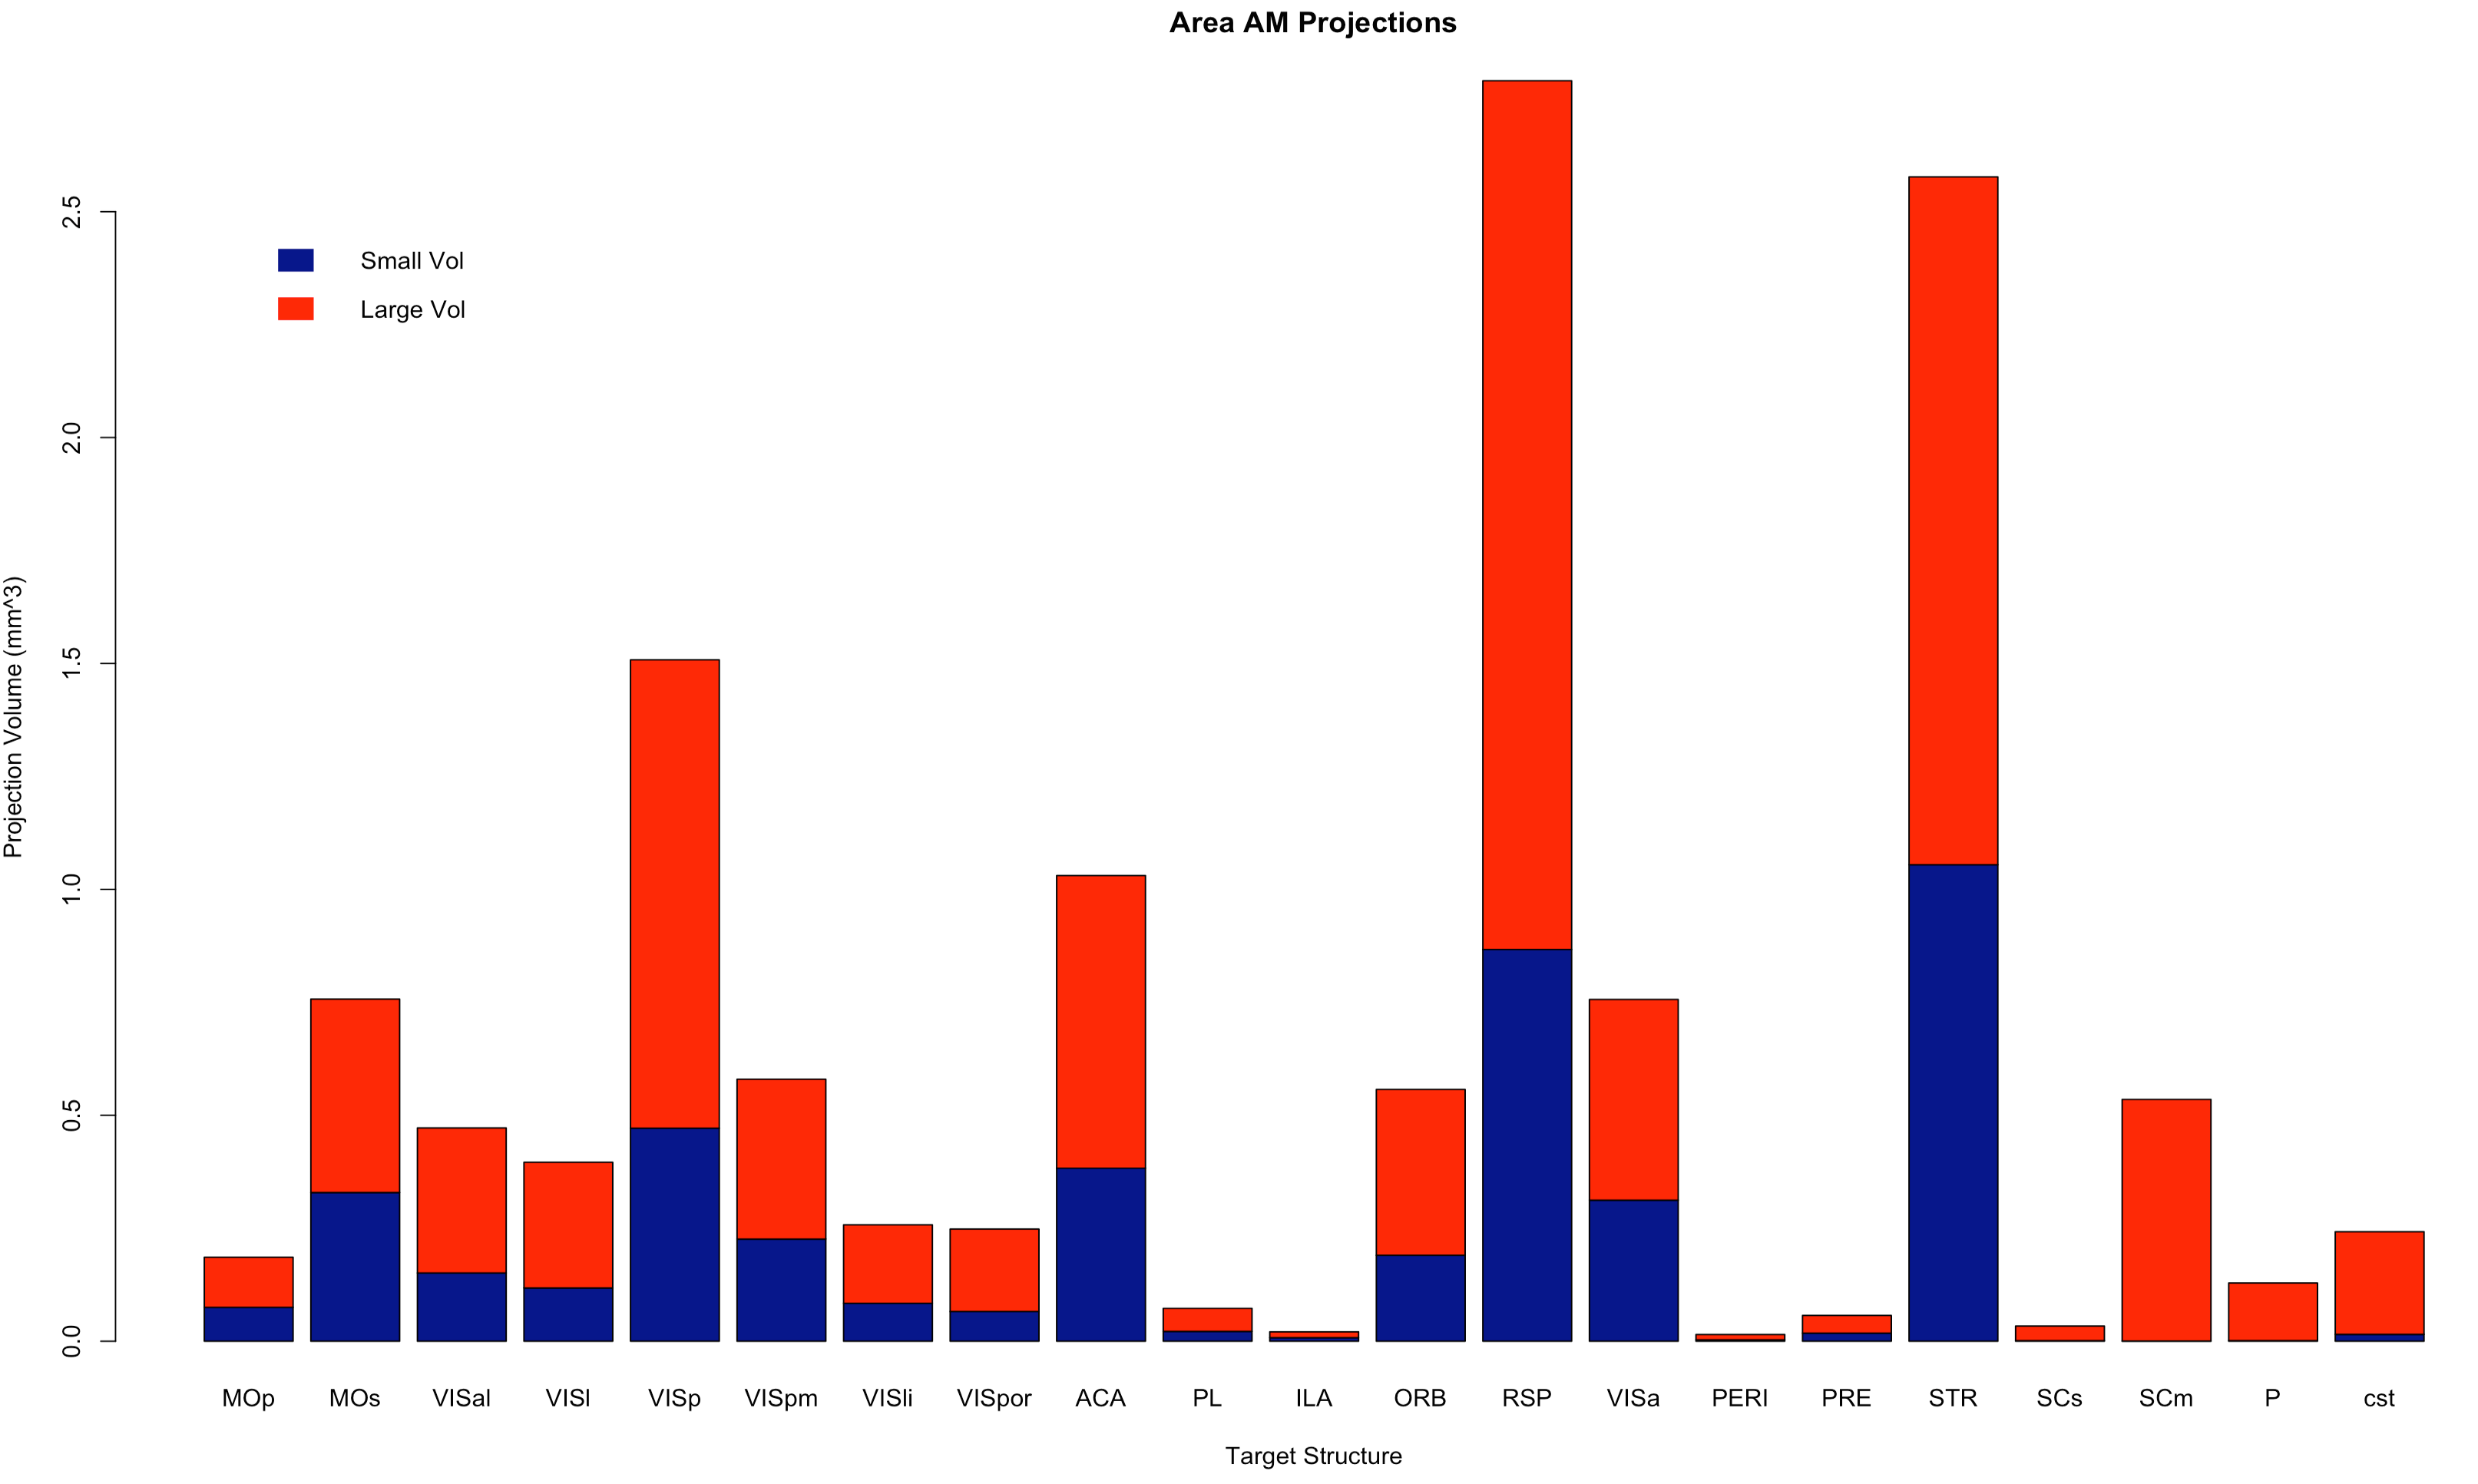
\includegraphics[width=\textwidth]{Figures/chapter4/areaAMprojectiondata2.png}
  \caption[Area AM Projection Target Data]{\textbf{Area AM Projection Target Data} Represented in a bar graph showing projection volume (sum of detected signal in mm\^3) at target structure for small (dark blue) and large (red) volume tracer injections. Data obtained from the Allen Institute Brain Connectivity Atlas \parencite{AllenBrain2015}; experiment id: 528510546 and 518742338.See list of abbreviations.}
   \label{fig:areaAMprojections}
\end{figure}

\section{General Experimental Strategy}
\subsection{Strategy for \emph{in vivo} optogenetic silencing of area AM}
The goal of the experiments in this chapter was to, reversibly, silence visual area AM as mice performed the visual pulses task. To this end, I employed an optogenetic strategy to silencing activity in area AM. Specifically, I used the cruxhalorhodopsin Jaws (or Halo57), a red light-driven chloride ion pump capable of powerful optogenetic inhibition \parencite{Chuong2014,Acker2016}. Another optogenetic approach that was explored in pilot experiments was to activate inhibitory neurons (PV+ or Gad2+)  optogenetic activator Channelrhodopsin (ChR2). Although cortical silencing through inhibitory neuron activation has been used to silence mouse visual cortex during behavior \parencite{Madisen2012,Glickfeld2013b,Poort2015,Burgess2016}, however this approach was incompatible with the widefield mapping of visual areas with GCaMP6 transgenic mice.\par
Details of the experimental procedures are described in Appendix \ref{AppendixA}. Briefly, area AM was identified in each mouse with widefield GCaMP6 imaging approach described in Chapter \ref{Chapter4}. Jaws was delivered into unilateral area AM through a viral construct with either a pan-neuronal promoter (human synapsin, hSyn, Group 1 mice) or excitatory neuron promoter (CamkII-$\alpha$, Group 2 mice). Optogenetic stimulation was randomly interleaved in 25\% of trials within a session. A linear downward ramp was added (Figure \ref{fig:AMgroup1summary} a) to the end of the optogenetic stimulus waveform to reduce the effect of rebound excitation that occurs during optogenetic inhibition \parencite{Chuong2014,Guo2014b}.
\begin{figure}
  \centering
   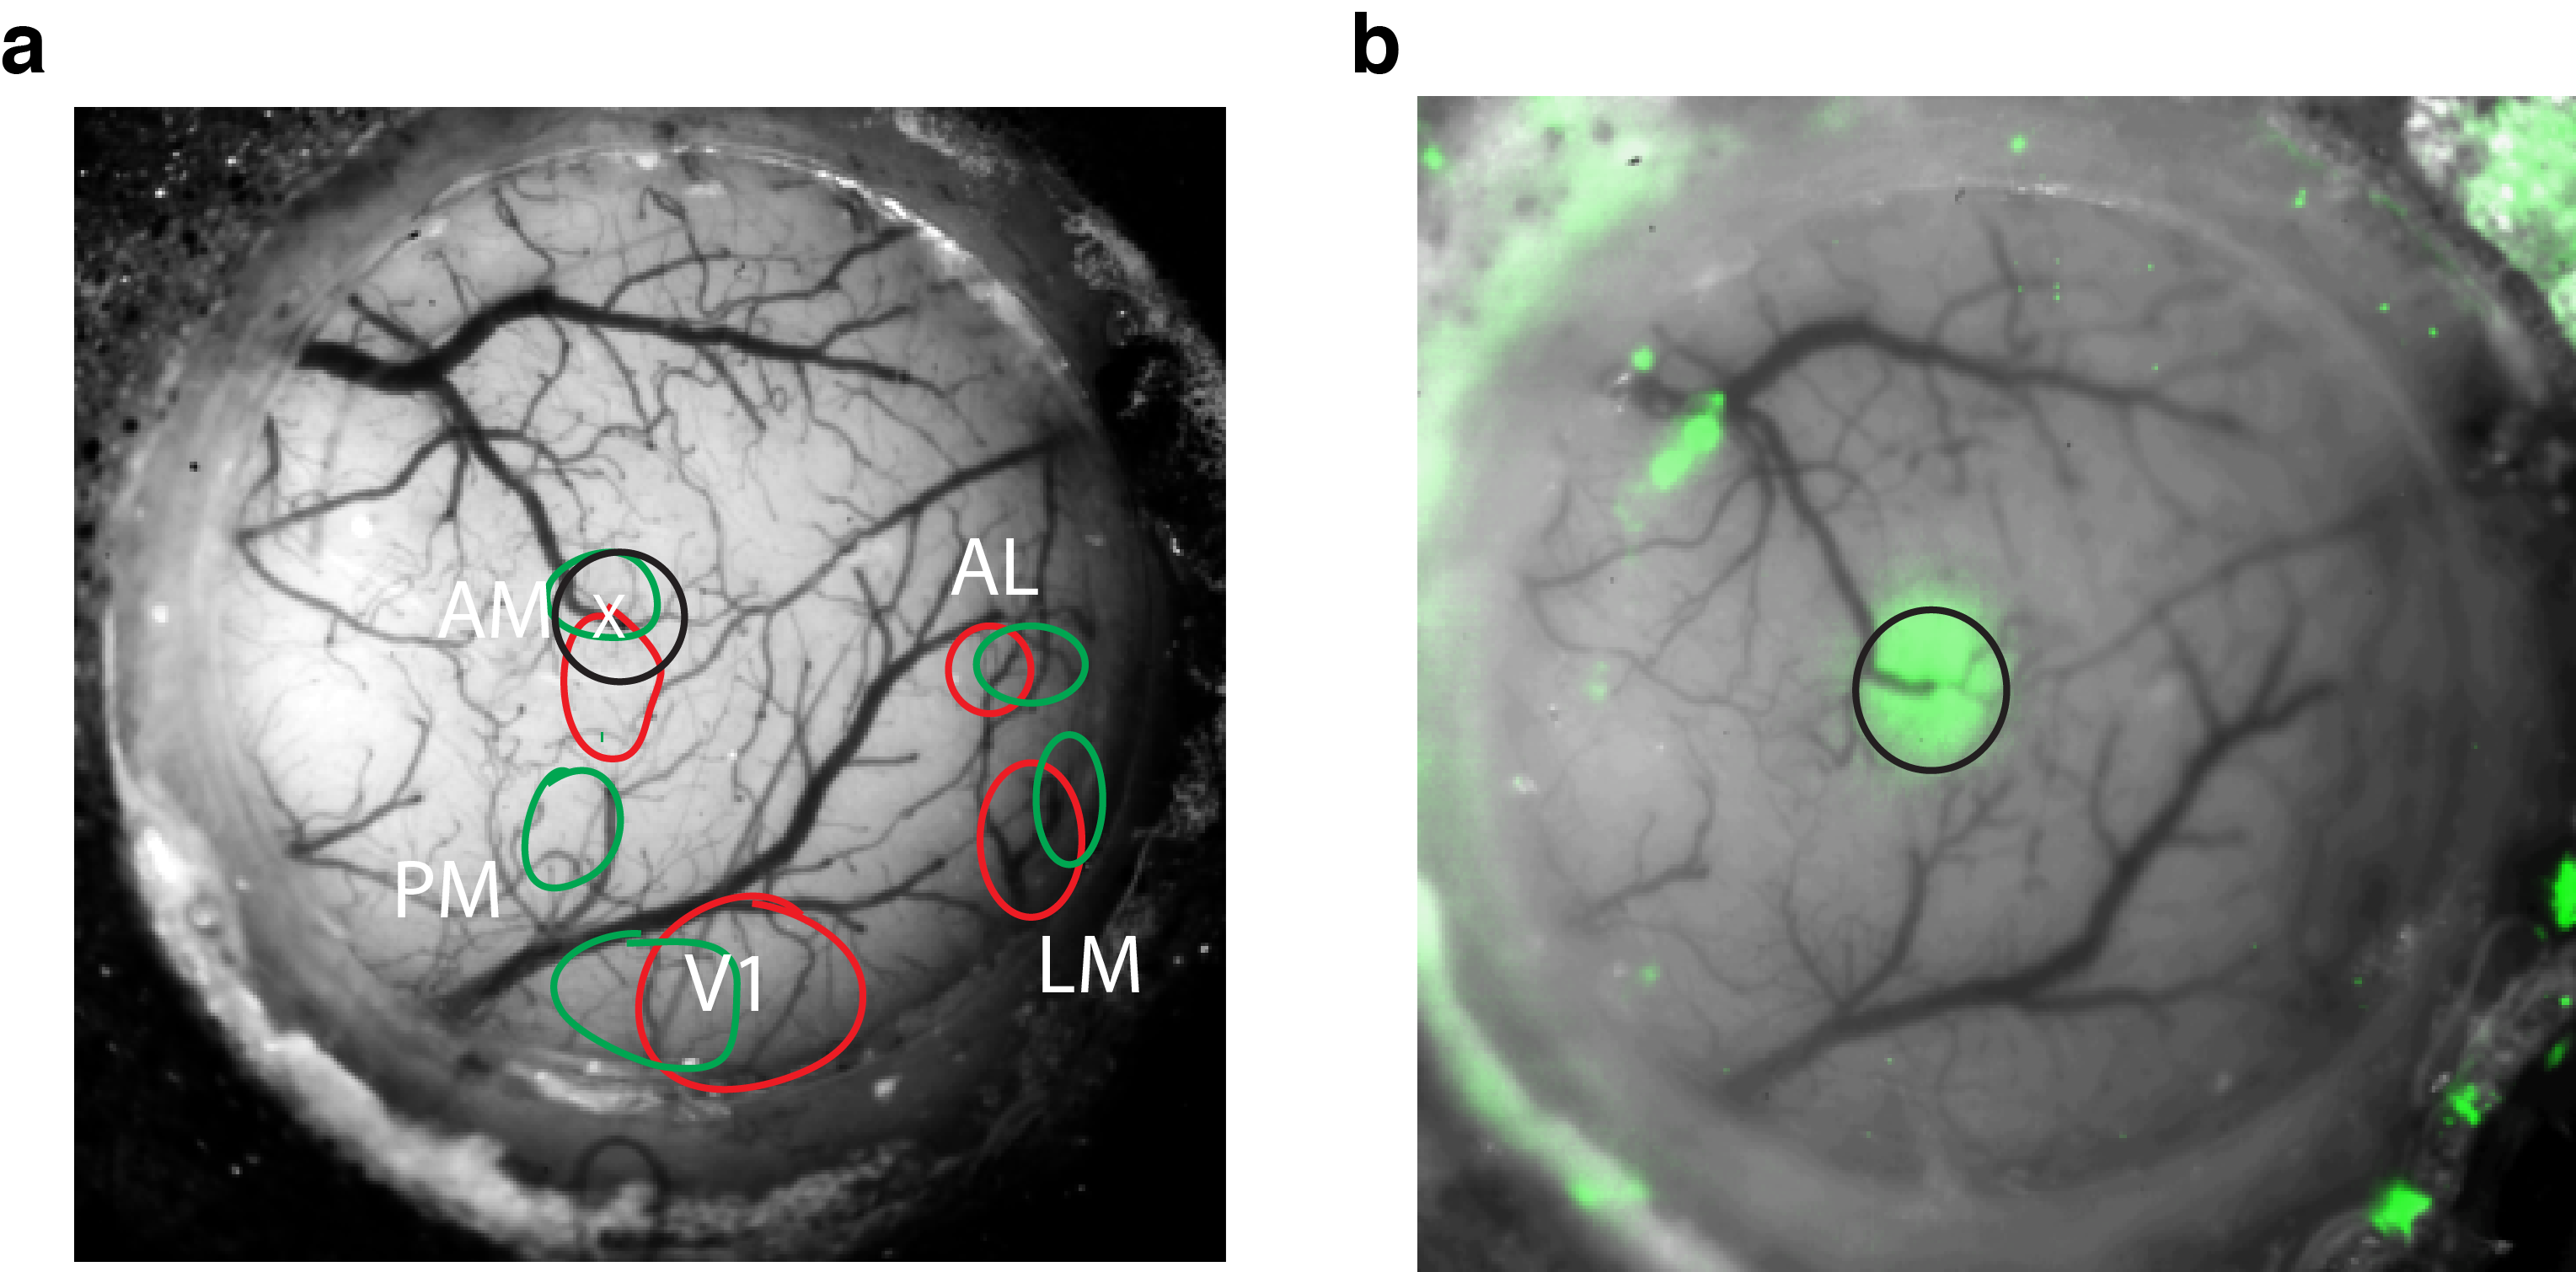
\includegraphics[width=\textwidth]{Figures/chapter4/kg07_jaws_gfp_expression.png}
  \caption[Jaws Virus Expression \emph{in vivo} in Area AM]{\textbf{Jaws Virus Expression \emph{in vivo} in area AM} (a) GCaMP6 response map overlay on optical window. Retinotopic map generated from response to drifting gratings (25$\deg$), 4Hz, 0.04 cycles/degree positioned at elevation of +15$\deg$ and azimuth 43$\deg$ (red) and 83$\deg$ (green). (b) Jaws-GFP expression (green) in area AM nine days post virus injection. }
   \label{fig:virusexp}
\end{figure}
%-----------------------------------------------------------------------
%------------------------------------------------------------------------
\subsection{Retinotopic Mapping of Visual Area AM}
Because of the small size of most visual areas including AM, their respective positions from bregma could vary from animal to animal; hence I performed retinotopic mapping in each mouse in order to target AM for viral delivery. To map visual areas, I imaged visually-evoked activity in awake transgenic mice expressing GCaMP6 in excitatory neurons (Ai95;Emx-cre and Ai93;ttA;Emx-cre) and generally employed one of two retinotopic mapping methods: spatially restricted gratings \parencite{Gias2005,Andermann2011} or periodic drifting bar \parencite{Sereno1995,Kalatsky2003}. The spatially-restricted gratings approach uses drifting gratings (25-40$\deg$ in diameter) positioned at different locations in the visual field (nasal vs. temporal or upper vs. lower). The gratings allow the experimenter to optimize the stimulus for the spatiotemporal frequency preferences of individual visual areas. Although this approach is easy to implement, in practice it requires many repetitions and high signal-to-noise to produce quality interpretable maps. The approach is not scalable because the maps need to be curated manually, and therefore not it was difficult to standardize across mice. Visual area AM was mapped using the grating procedure in a subset of mice (Figure \ref{fig:virusexp}, Group 1 below). \par 

I found the Fourier drifting bar methods to be a more consistent and scalable retinotopic mapping approach. Technical details and procedures for implementing the approach are described in \parencite{Kalatsky2003,Juavinett2016}. Briefly, a bar is periodically drifted across the screen in the 4 cardinal direction. Since the bar drifts at a fixed frequency, 
Fourier decomposition (Fast Fourier Transform) is used to isolate the phase at the bar drift (or stimulation) frequency. Phase maps are generated for the horizontal and vertical bar drift directions, which correspond to altitude and azimuth visual space (Figure \ref{fig:retinomap} a, b). Using a clever mathematical trick, visual field sign maps (Figure \ref{fig:retinomap}c) are generated by taking the sine of the difference between the gradients for the altitude and azimuth maps \parencite{Sereno1994,Garrett2014}. Borders between visual areas are defined With the visual field sign map (Figure \ref{fig:retinomap}d). I implemented this approach in awake head-fixed mice who were passively viewing the stimulus. The mice were free to walk on a wheel. \par 

\subsection{Statistical Analysis of Behavioral Performance}
The performance was visualized with the 4-parameter psychometric function described in Chapter \ref{Chapter2}. However, to statistically test whether there was a significant effect of photoinhibition of area AM on the population group level, I used a Generalized Linear Mixed-Model (GLMM). GLMMs are an extension of the Generalized Linear Model, which can be used to model both fixed and random effects in categorical data. In psychophysics, GLMMs can be used to generalize results across multiple subjects and experimental conditions \parencite{KnoblauchMaloney2012,Moscatelli2012a,Erlich2015}. \\The GLMM model written in the Wilkinson notation:
\begin{equation}
	\centering
	r \sim  1 + evidence + opto + evidence:opto + (evidence|subject/opto)
    \label{GLMM}
\end{equation}
Each term of the equation has a coefficient, $\beta$. The model specifies that the subject's response, \emph{r}, is a function of the fixed effects: intercept, the \emph{evidence} which represents the slope of the psychometric function is defined as the difference between the flash rate and the category boundary, the photoinhibition indicator variable \emph{opto}, and the interaction between the \emph{evidence} and \emph{opto}. The interaction term \emph{evidence:opto} evaluates whether photoinhibition alters the subject's sensitivity or the slope of the psychometric function. The model allows the four fixed effects parameters to vary for each individual subject (random effects). The model uses a probit linking function and was fit using a Maximum Likelihood procedure. The GLMM analysis was performed using the R package 'lme4' and is identical to the analysis used by \textcite{Erlich2015}. \par 

The effect of photoinhibition on the horizontal location of the psychometric function was quantified by the choice bias (Figure \ref{fig:amGLMMparams}b). The choice bias was defined as: 
\begin{equation}
	\centering
	choice\quad bias =  \frac{\beta_{opto}}{\beta_{evidence}+\beta_{evidence:opto}}
    \label{choicebias}
\end{equation}
Where $\beta_{opto}$, $\beta_{evidence}$, $\beta_{evidence:opto}$ are estimated coefficients from the GLMM (Equation \ref{GLMM}). The choice bias reflects the equivalent change in the stimulus that would recapitulate the observed effects of photoinhibition and is in units of flashes/s. Positive choice bias would indicate that on photoinhibition trials caused the subject to be biased towards high-rate responses. Because the choice bias is computed from estimated parameters of the GLMM model, I used error propagation to compute the errors (95\% confidence intervals, CI).

%----------------------------------------------------------------------------------
\begin{figure}
  \centering
   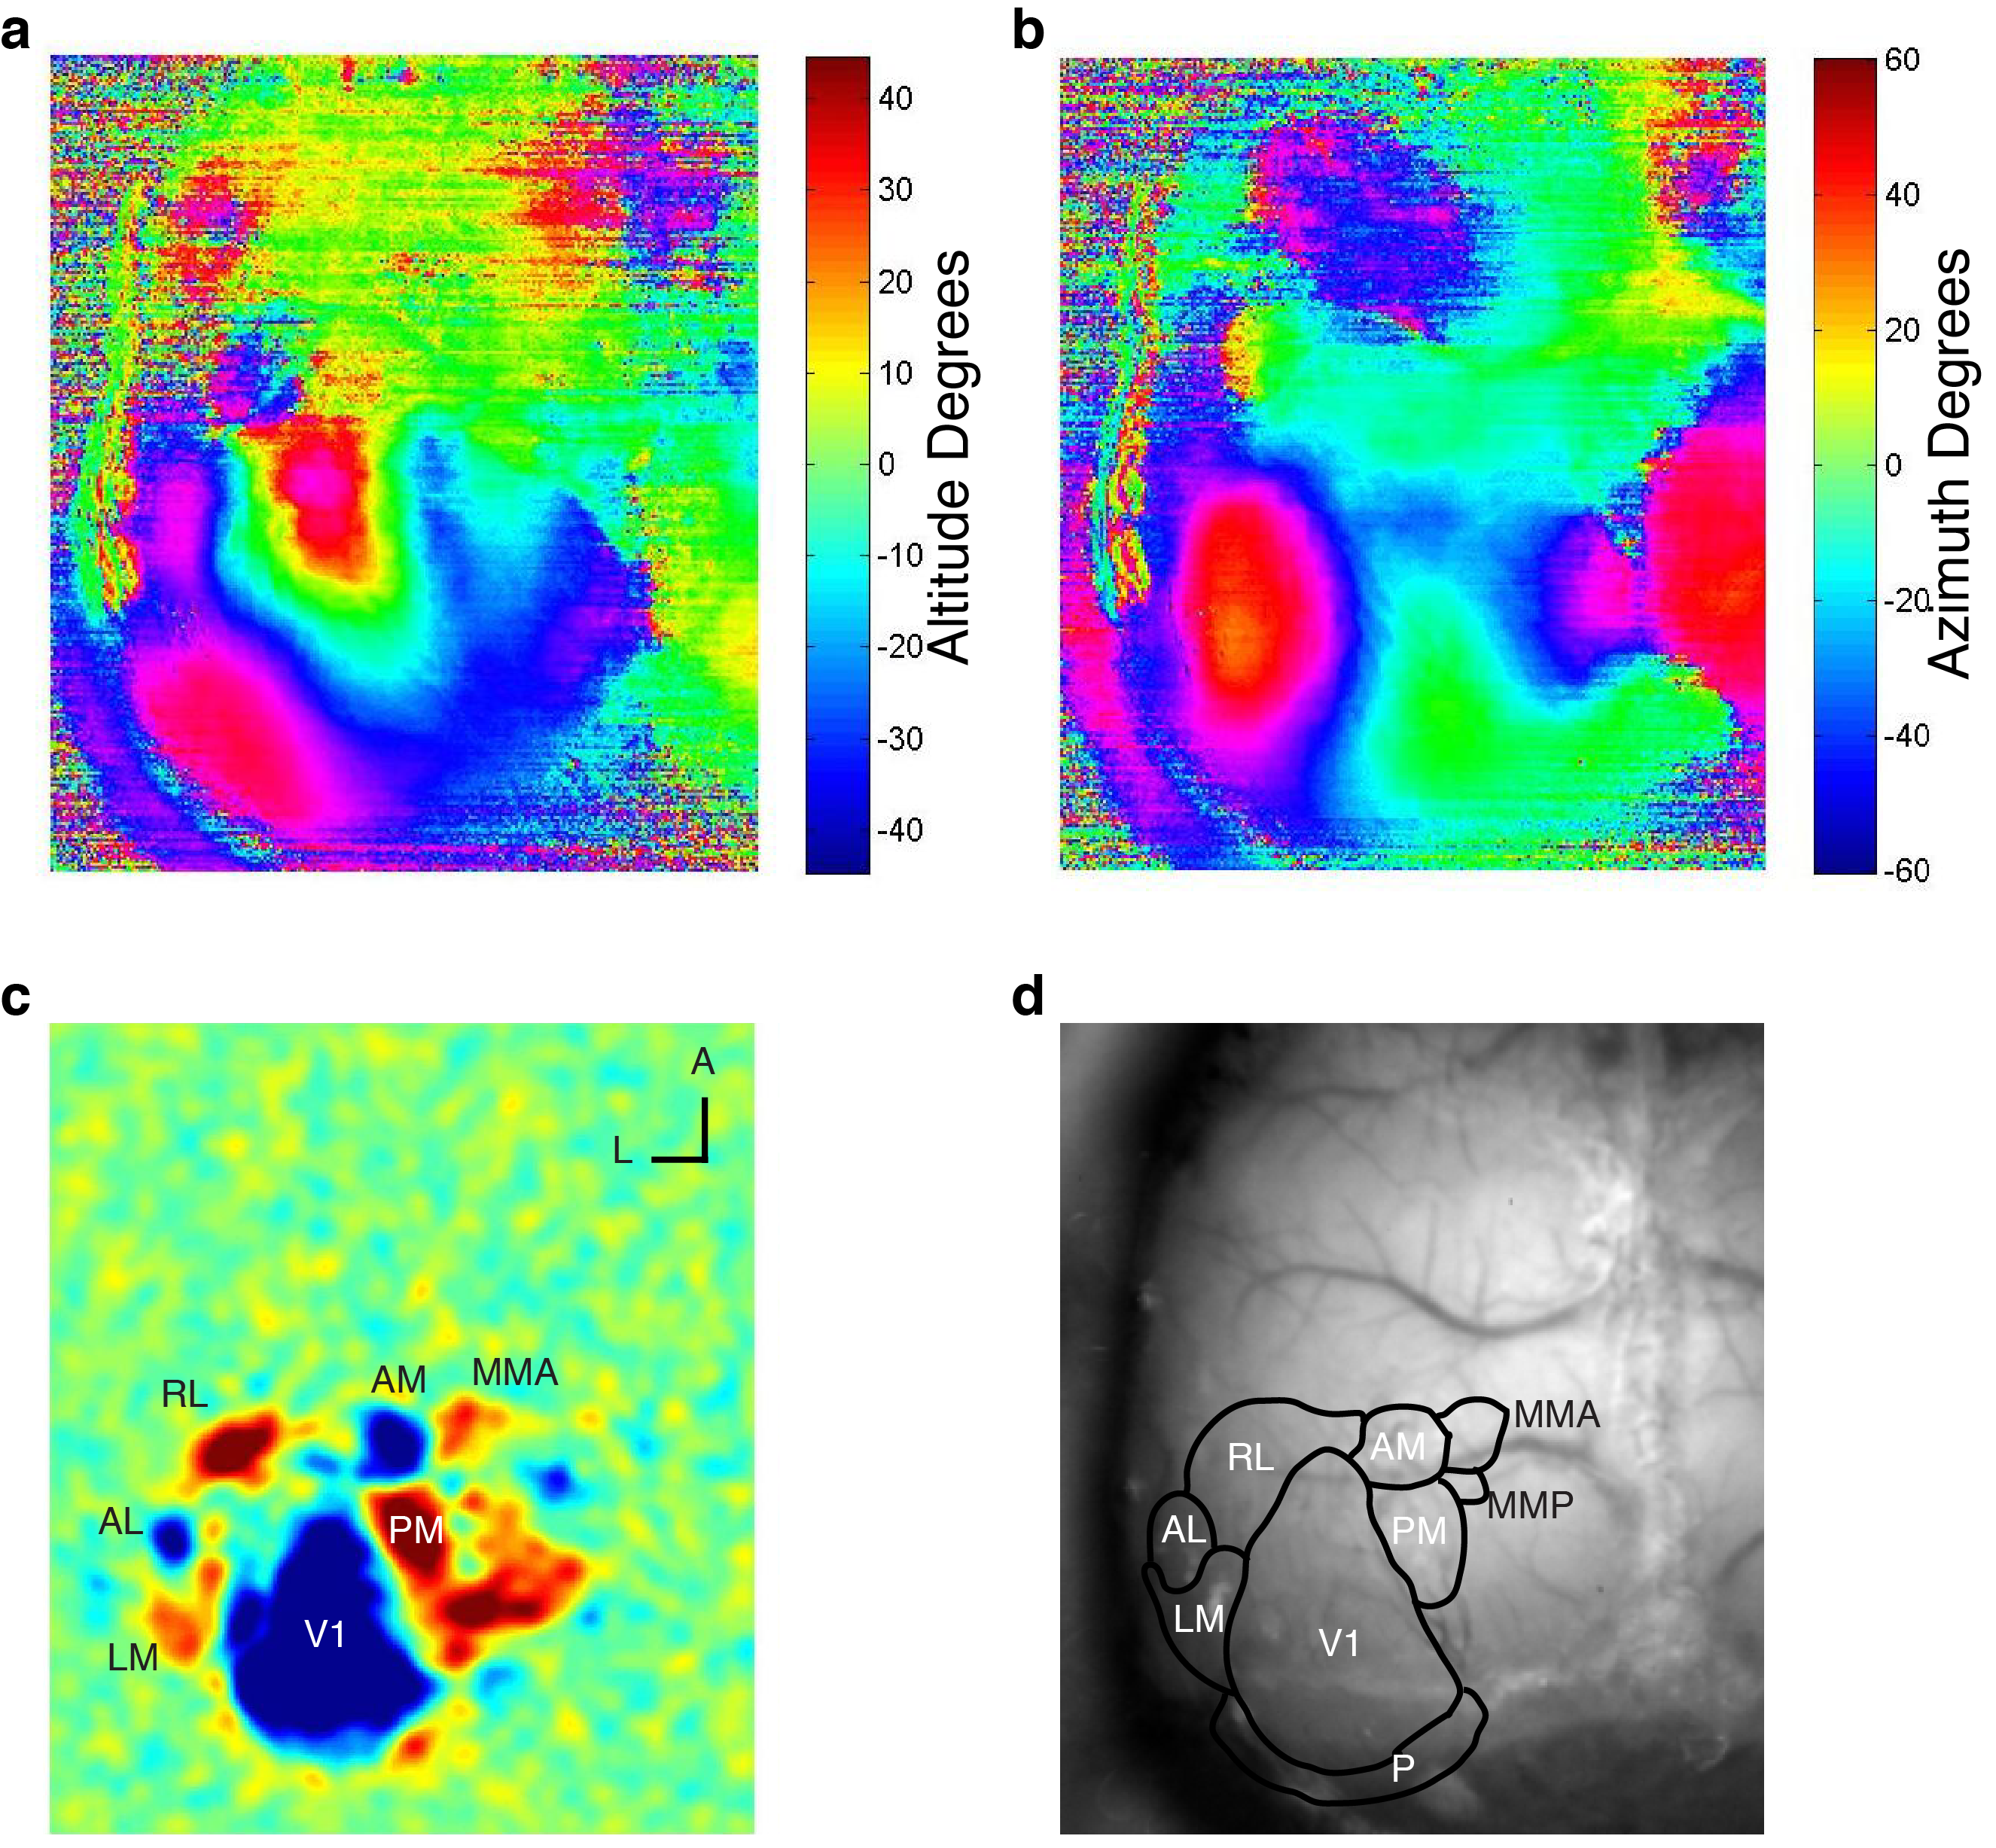
\includegraphics[width=\textwidth]{Figures/chapter4/retino_maps.png}
  \caption[Example Retinotopic Map of Mouse Visual Areas]{\textbf{Example Retinotopic Map of Mouse Visual Areas}. (a) Altitude and (b) Azimuth phase map (c) Visual field sign map with labeled visual areas (d) Overlay of visual areas borders on skull. Borders drawn by hand with visual field sign map.}
   \label{fig:retinomap}
\end{figure}
%---------------------------------------------------------------------------
%-------------------------------------------------------------------------------
\section{Predicted Consequences of Unilateral Inhibition of Visual Area AM}
Since the behavioral consequences of inhibiting mouse secondary visual areas are largely unknown, let us consider the potential behavioral outcomes of optogenetic inhibition of area AM (Figure \ref{fig:predictions}). Several outcomes are possible including, (a) a shift in choice bias, (b) a change in sensitivity, (c) a combination of changes in sensitivity and bias, or (d) no effect. 

Photoinhibition of AM could cause a horizontal shift in the psychometric function (Figure \ref{fig:predictions}a), which would indicate either a sensory bias towards a stimulus category (i.e. low- or high-rate) or a spatial bias towards a response port (i.e. left or right-hand port). A sensory bias could occur if AM selectively preferred low- or high-rate stimuli. This is an attractive viewpoint given that higher-order visual areas in the mouse have distinct preferences for temporal frequency \parencite{Andermann2011,Marshel2011,Tohmi2014}. However, it is not clear whether these preferences extend to stochastic (i.e. non-periodic) sequences of flashes and more so, how visual areas represent the visual pulses stimuli remains an open question. Alternatively, AM is in a position to mediate a spatial bias. It is reciprocally connected with cortical \parencite{Wang2012} and subcortical motor areas \parencite{AllenBrain2015} (Figure \ref{fig:areaAMprojections}), which are capable of biasing movements. Recently, \textcite{Znamenskiy2013b} showed that manipulation of corticostriatal projections in rat selectively biased choices in an auditory evidence accumulation task. 

Photoinhibition of AM could reduce sensitivity (Figure \ref{fig:predictions}b). Since area AM is a retinotopic visual area, it could also be involved in the processing of the visual flashes stimulus in a manner that informs computation of the choice downstream. Therefore inhibition of area AM could affect the slope of the psychometric curve, i.e. the subject's sensitivity. Reduced sensitivity would be consistent with results presented in the previous chapter (Chapter \ref{Chapter3}), and previous studies in rat PPC \parencite{Raposo2014,Licata2017}. 

While manipulation of AM could produce shifts in sensitivity and/or changes in bias, the manipulation may also have no behavioral consequence o
in the visual pulses task either because the neural activity in area AM does not contribute to the behavior or because unilateral silencing is not sufficient to disrupt the behavior. In the latter case, the opposite hemisphere is still intact and may compensate for the loss of unilateral activity \parencite{Li2016}. The scenario is plausible since the animals are presented with full- field visual flashes and presumably, information comes in to both eyes and, by extension, both hemispheres of AM.

%-----------------------------------------------------------------------------
\begin{figure}
  \centering
   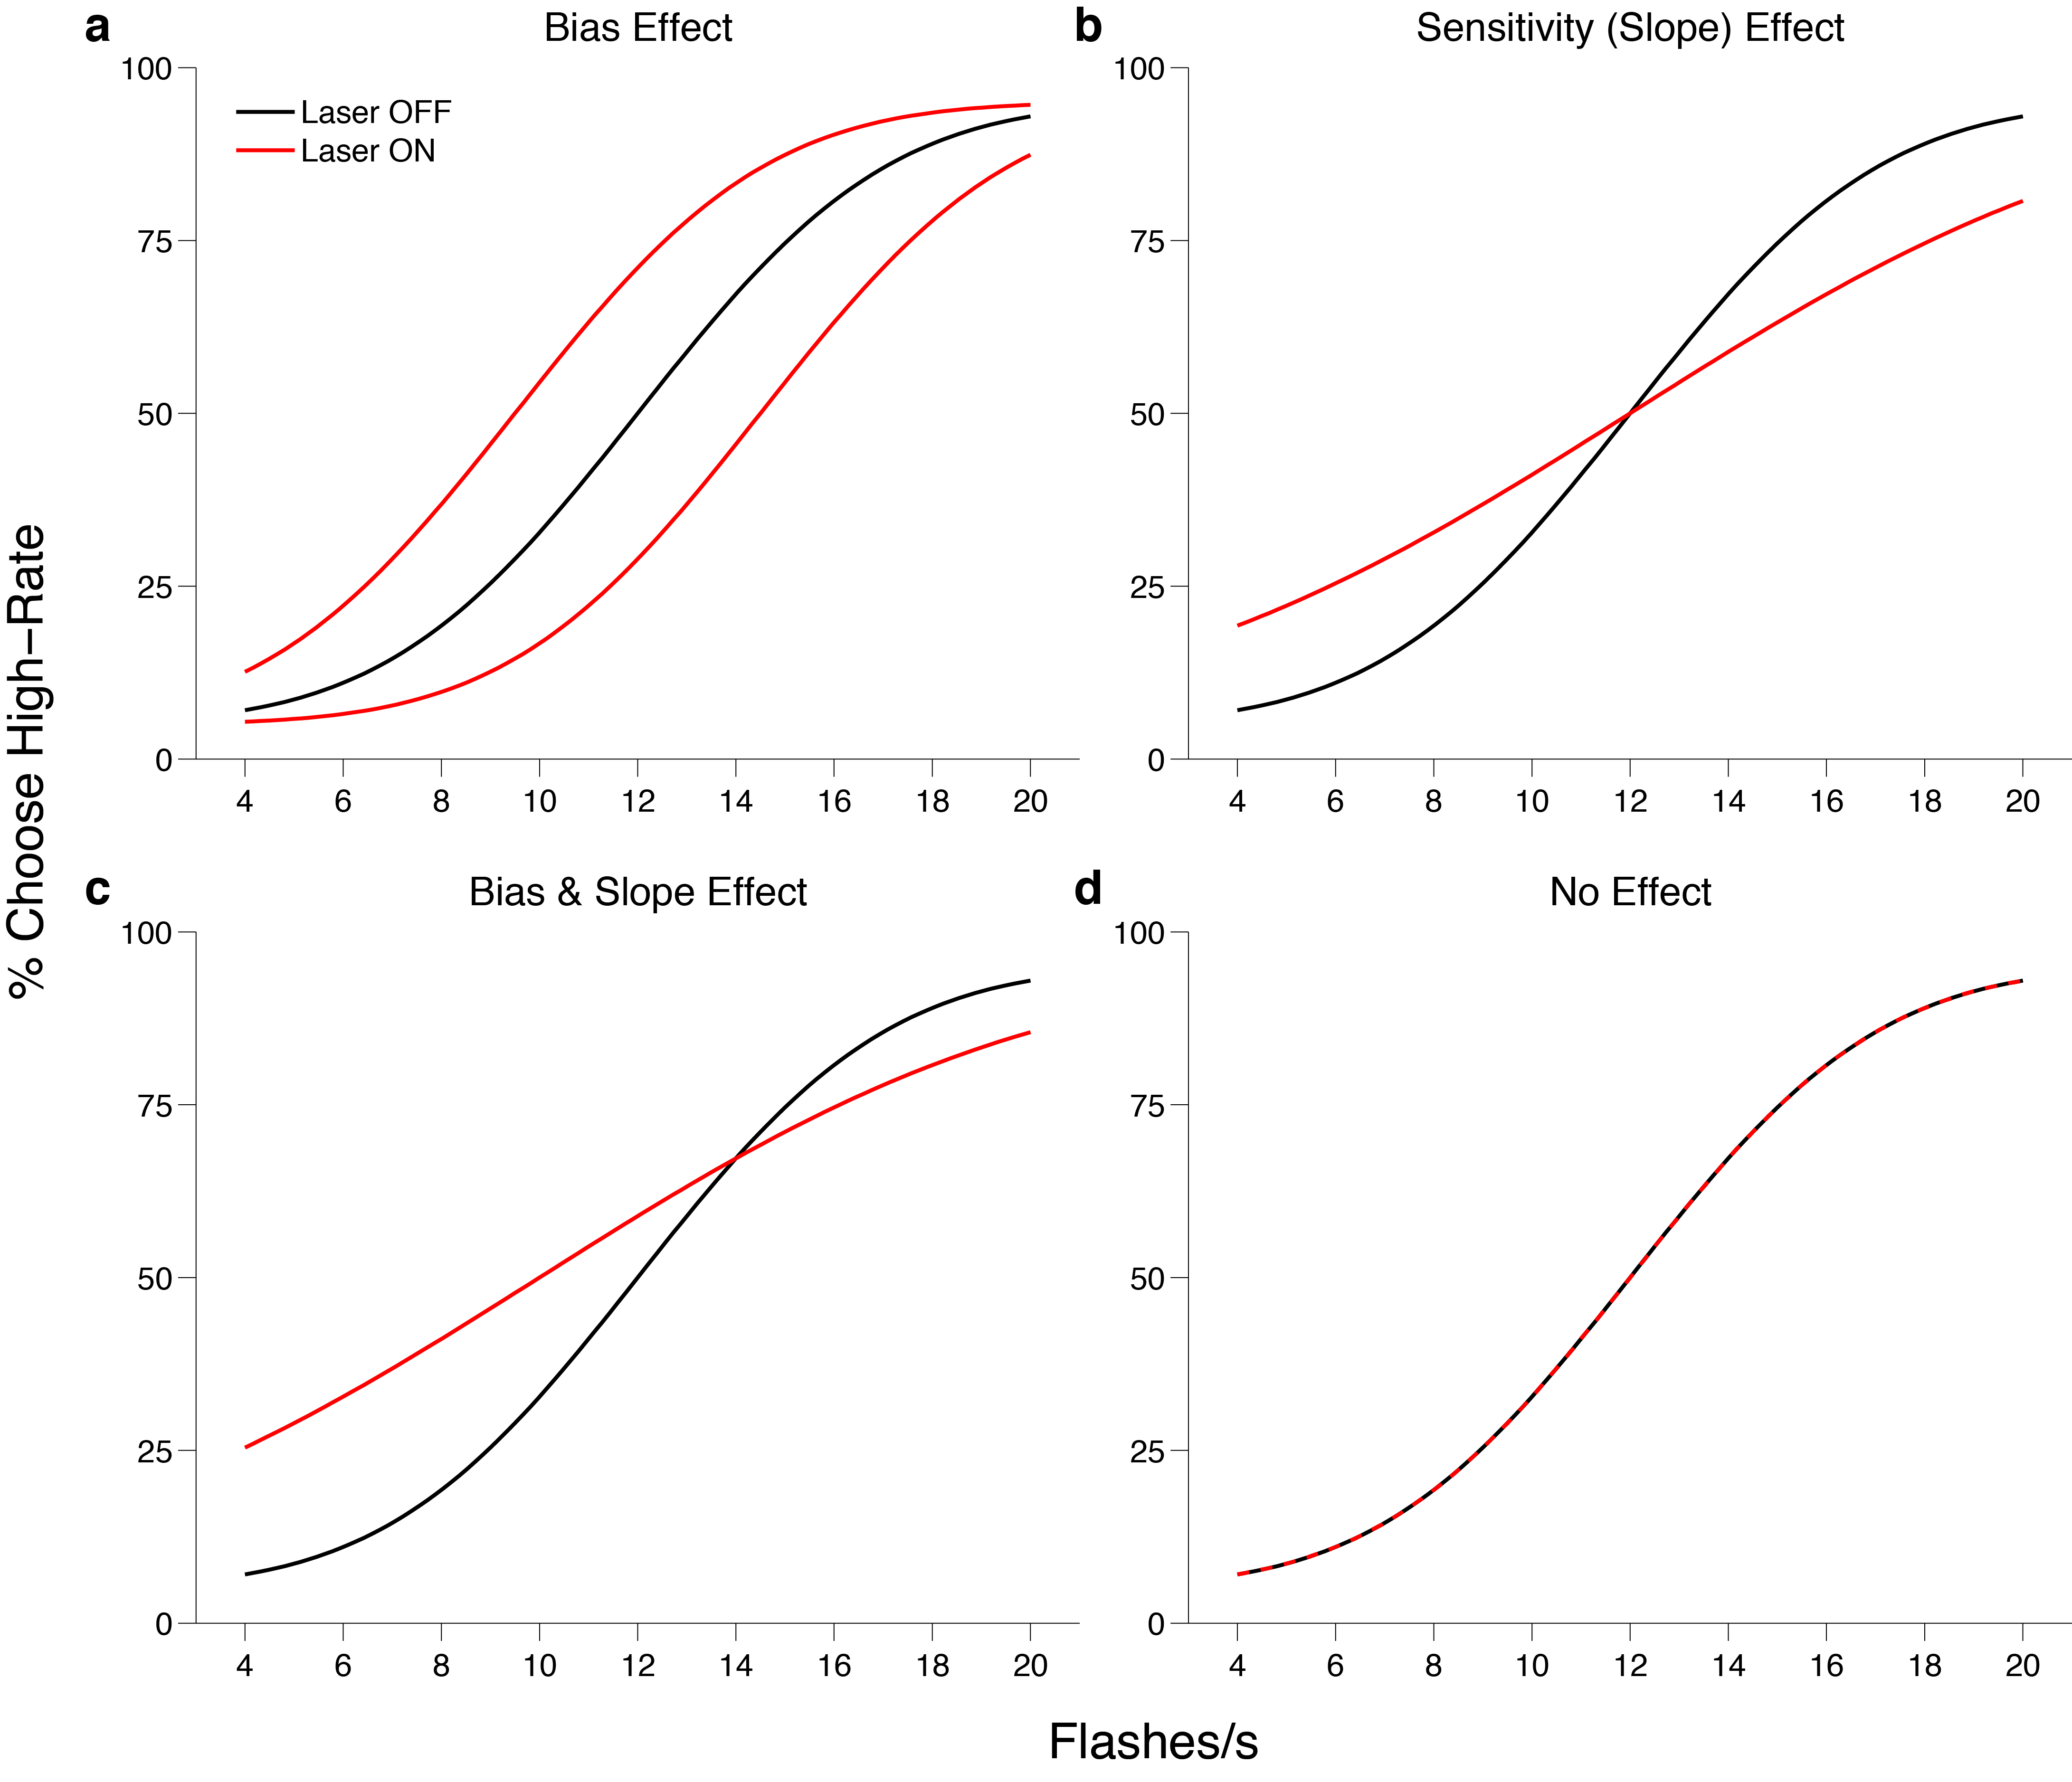
\includegraphics[width=\textwidth]{Figures/chapter4/pmfPredictions.png}
  \caption[Schematic of Potential Behavioral Outcomes of Optogenetic Inhibition]{\textbf{Schematic of Potential Behavioral Outcomes of Optogenetic Inhibition} Optogenetic inhibition of visual area AM could potentially cause: (a) horizontal shift in the psychometric function, (b) change in slope i.e. sensitivity, (c) both shift in bias and change in sensitivity, or (d) no effect.}
   \label{fig:predictions}
\end{figure}
%-----------------------------------------------------------------------------
\section{Results}
\subsection{Area AM Inhibition - Group 1}
The first group of mice (Figures \ref{fig:AMgroup1summary}, \ref{fig:AMgroup1individual}, and \ref{fig:AMg1GLMM32}, n = 6 mice, Ai95;Emx-cre) were injected with Jaws in the right hemisphere and were trained with the standard contingency (Low-rate go LEFT and High-rate go RIGHT). Photoinhibition occurred randomly on 25\% of trials, at an irradiance of 32 mW/mm$^{2}$. On laser ON trials, all mice in this group exhibited an increased tendency to make more high-rate choices (Figures \ref{fig:AMgroup1summary}, \ref{fig:AMgroup1individual}, and \ref{fig:AMg1GLMM32}), as indicated by a leftward shift of the psychometric function on photoinhibition trials (red) compared to control trials (black). The observed bias had the equivalent effect of adding more flashes (choice bias = 3.47 flashes/s [2.46 4.54] 95\% CI), as quantified by Equation \ref{choicebias}. AM photoinhibition also caused a significant decrease in the animals' sensitivity, as indicated by a decrease in the slope of the psychometric function on Laser ON trials (GLMM Test, $\beta_{evidence:opto}$ = -0.021 [-0.034, -0.0085] 95\% CI, p=0.0011). The change is equivalent to a 16.58\% reduction in the slope on Laser ON compared to Laser OFF trials. The combined effect of the horizontal shift and reduced sensitivity is consistent the predictions made in Figure \ref{fig:predictions}c and in line with the anatomical and functional properties of AM. Therefore the results thus far lend support for the role of visual area AM in visually-guided decision making. \par 

The observed bias could be a result of either a sensory, high-rate, bias or a spatial bias towards the ipsilateral hemifield in the direction of the optogenetic stimulation site. Therefore, based on this experiment alone the animals could have either a sensory (perceptual) bias towards high rate stimuli or a spatial (or motor) bias towards the right hemifield, ipsilateral to the implanted site. Plausible experiments that could disentangle these two hypotheses include (A) photoinhibition of the opposite hemisphere under the same behavioral contingency (Low-rate, go LEFT and High-Rate, go RIGHT) or (B) photoinhibition of the same hemisphere and and a reversed behavioral contingency (Low-rate, go RIGHT and High-Rate, go LEFT).\par

%-----------------------------------------------------------------------------
\begin{figure}
  \centering
   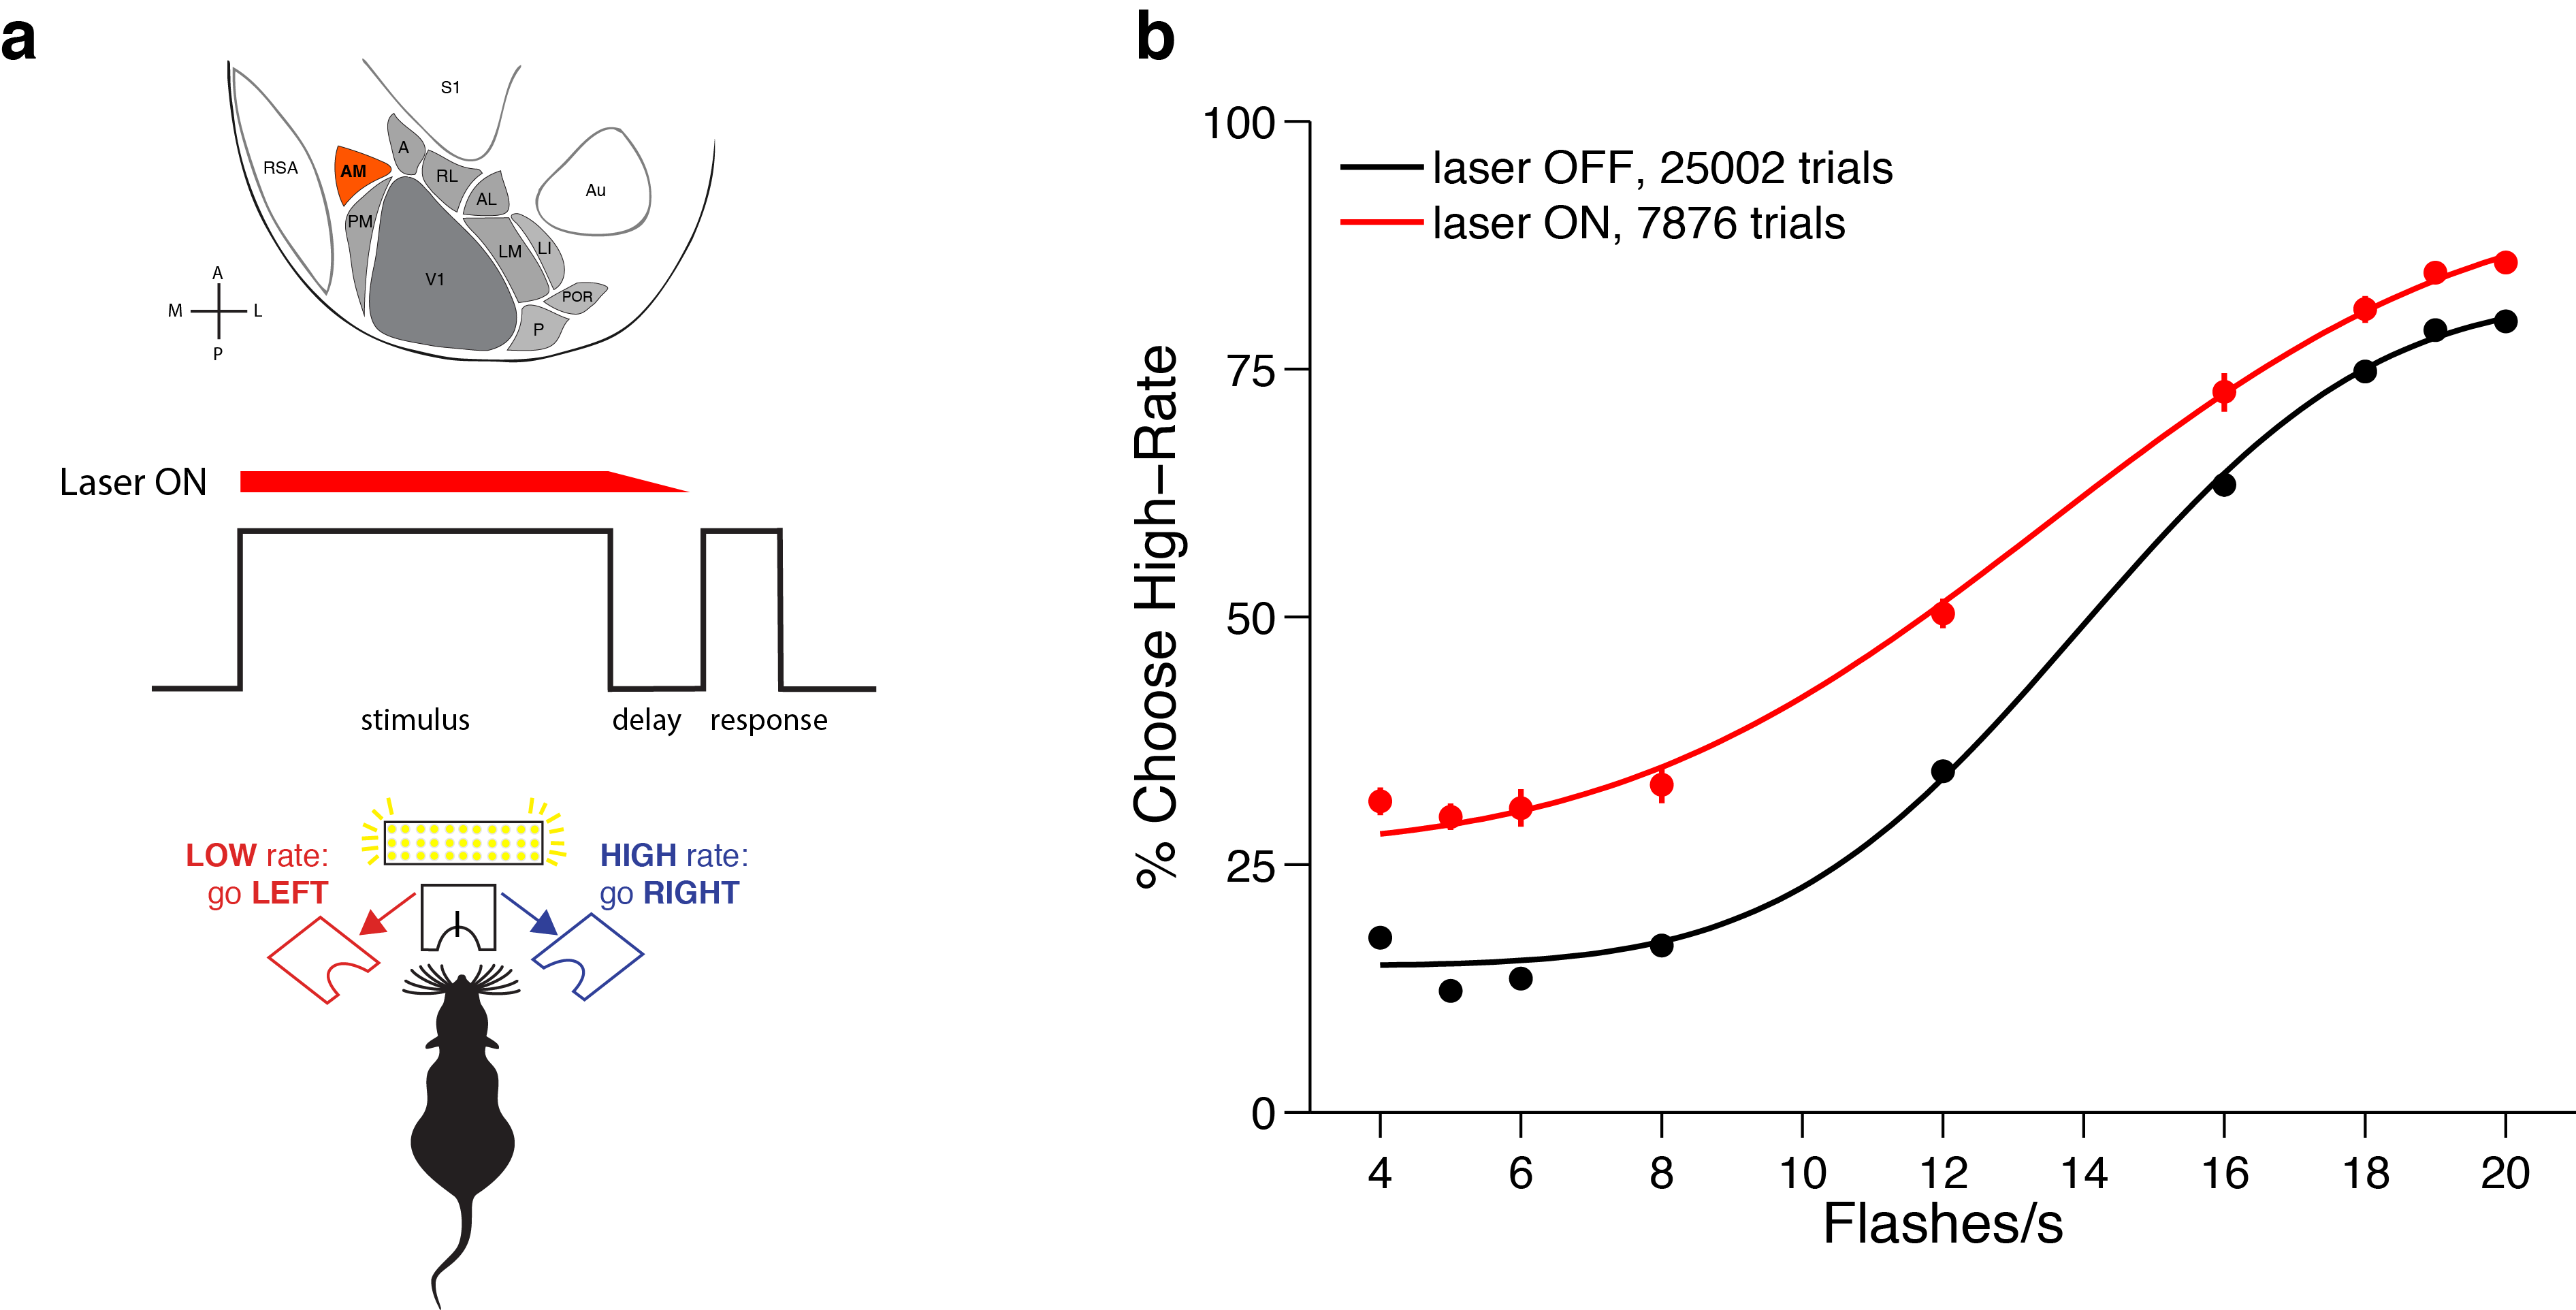
\includegraphics[width=\textwidth]{Figures/chapter4/jaws_AM_group1_summaryPMF.png}
  \caption[Area AM Group 1 Summary Psychophysical Data]{\textbf{Area AM Group 1 Summary Psychophysical Data} (a) Schematic of experimental configuration for group 1 animals.(b) Psychometric data of mice (n = 6) on laser OFF (black) and laser ON (red) trials (irradiance at 32 mW/mm$^{2}$). Circles represent psychometric performance at each event rate and the solid line is the psychometric function fit with a cumulative Normal (Equation \ref{eq:normalpmf}). Errors bars represent Wilson binomial confidence intervals on the psychometric data.}
   \label{fig:AMgroup1summary}
\end{figure}

%-----------------------------------------------------------------------------
%-----------------------------------------------------------------------------
\subsection{\emph{In Vivo} Red Light Stimulation Control Group}
The observation that inhibition of area AM increased the tendency to make high-rate choices could potentially explained by an artifact of the red light optogenetic stimulation, such that the mice are biased towards the red light delivered through the unilateral implanted optical fiber. Compared to short wavelength light such as blue and green, red light scatters minimally in tissue and is therefore able to travel several millimeters from the fiber implant site through the mouse's eyes \parencite{Danskin2015}.\par

To test whether this artifact contributed to behavioral effects observed in Group 1, I repeated the experiment in a new group of mice that were not injected with Jaws. Instead, the mice were injected with a sham virus (AAV-GFP) in area AM and implanted with an optical fiber. If the red light stimulation alone has no effect on the behavior, there would be no difference in the psychometric function (Figure \ref{fig:predictions} d; however, if the red light stimulation alone causes an artifact such as light directly activating the retina from within the brain \parencite{Danskin2015}, then the change in the psychometric curve would be similar to that observed in Group 1. \par

\emph{In vivo} red light stimulation of the control group resulted in behavioral effects (Figures \ref{fig:ctrlsummary} a and \ref{fig:ctrlindividual} a,c) similar to group 1. This observation is consistent with the idea that the red light alone introduces an artifact in the behavior, possibly due to red light escaping through eyes. However, the observed behavioral artifact in the controls does not rule out the possibility that unilateral inhibition of area AM inhibition does not have an effect on the behavior as observed in group 1 mice. The solution proposed by  \textcite{Danskin2015} to eliminate the behavioral artifact caused by \emph{in vivo} red light stimulation was to adapt the retina with dim white light near the eyes. However, application of this solution was maladaptive on the visual pulses task, as it reduced the subject's overall sensitivity and performance on the visual pulses task. \par

A solution that did not interfere with the subject's performance was to install red light within the behavior booth (Figure \ref{fig:mousehouselight} b). The external house red lights served to mask the red light escaping through the eyes and implant margins (Figure \ref{fig:mousehouselight} a), thereby making the mice less sensitive to the perception of red light. The artifact caused by \emph{in vivo} red light stimulation was greatly reduced by the presence of the house red lights (Figure \ref{fig:ctrlsummary}b, \ref{fig:ctrlindividual} b,d, and \ref{fig:glmmcontrol}), although it did not completely eliminate the artifact when the mice were again tested with more flash rates (Figures \ref{fig:ctrlpmfs}). 
%-----------------------------------------------------------------------------
\begin{figure}
  \centering
   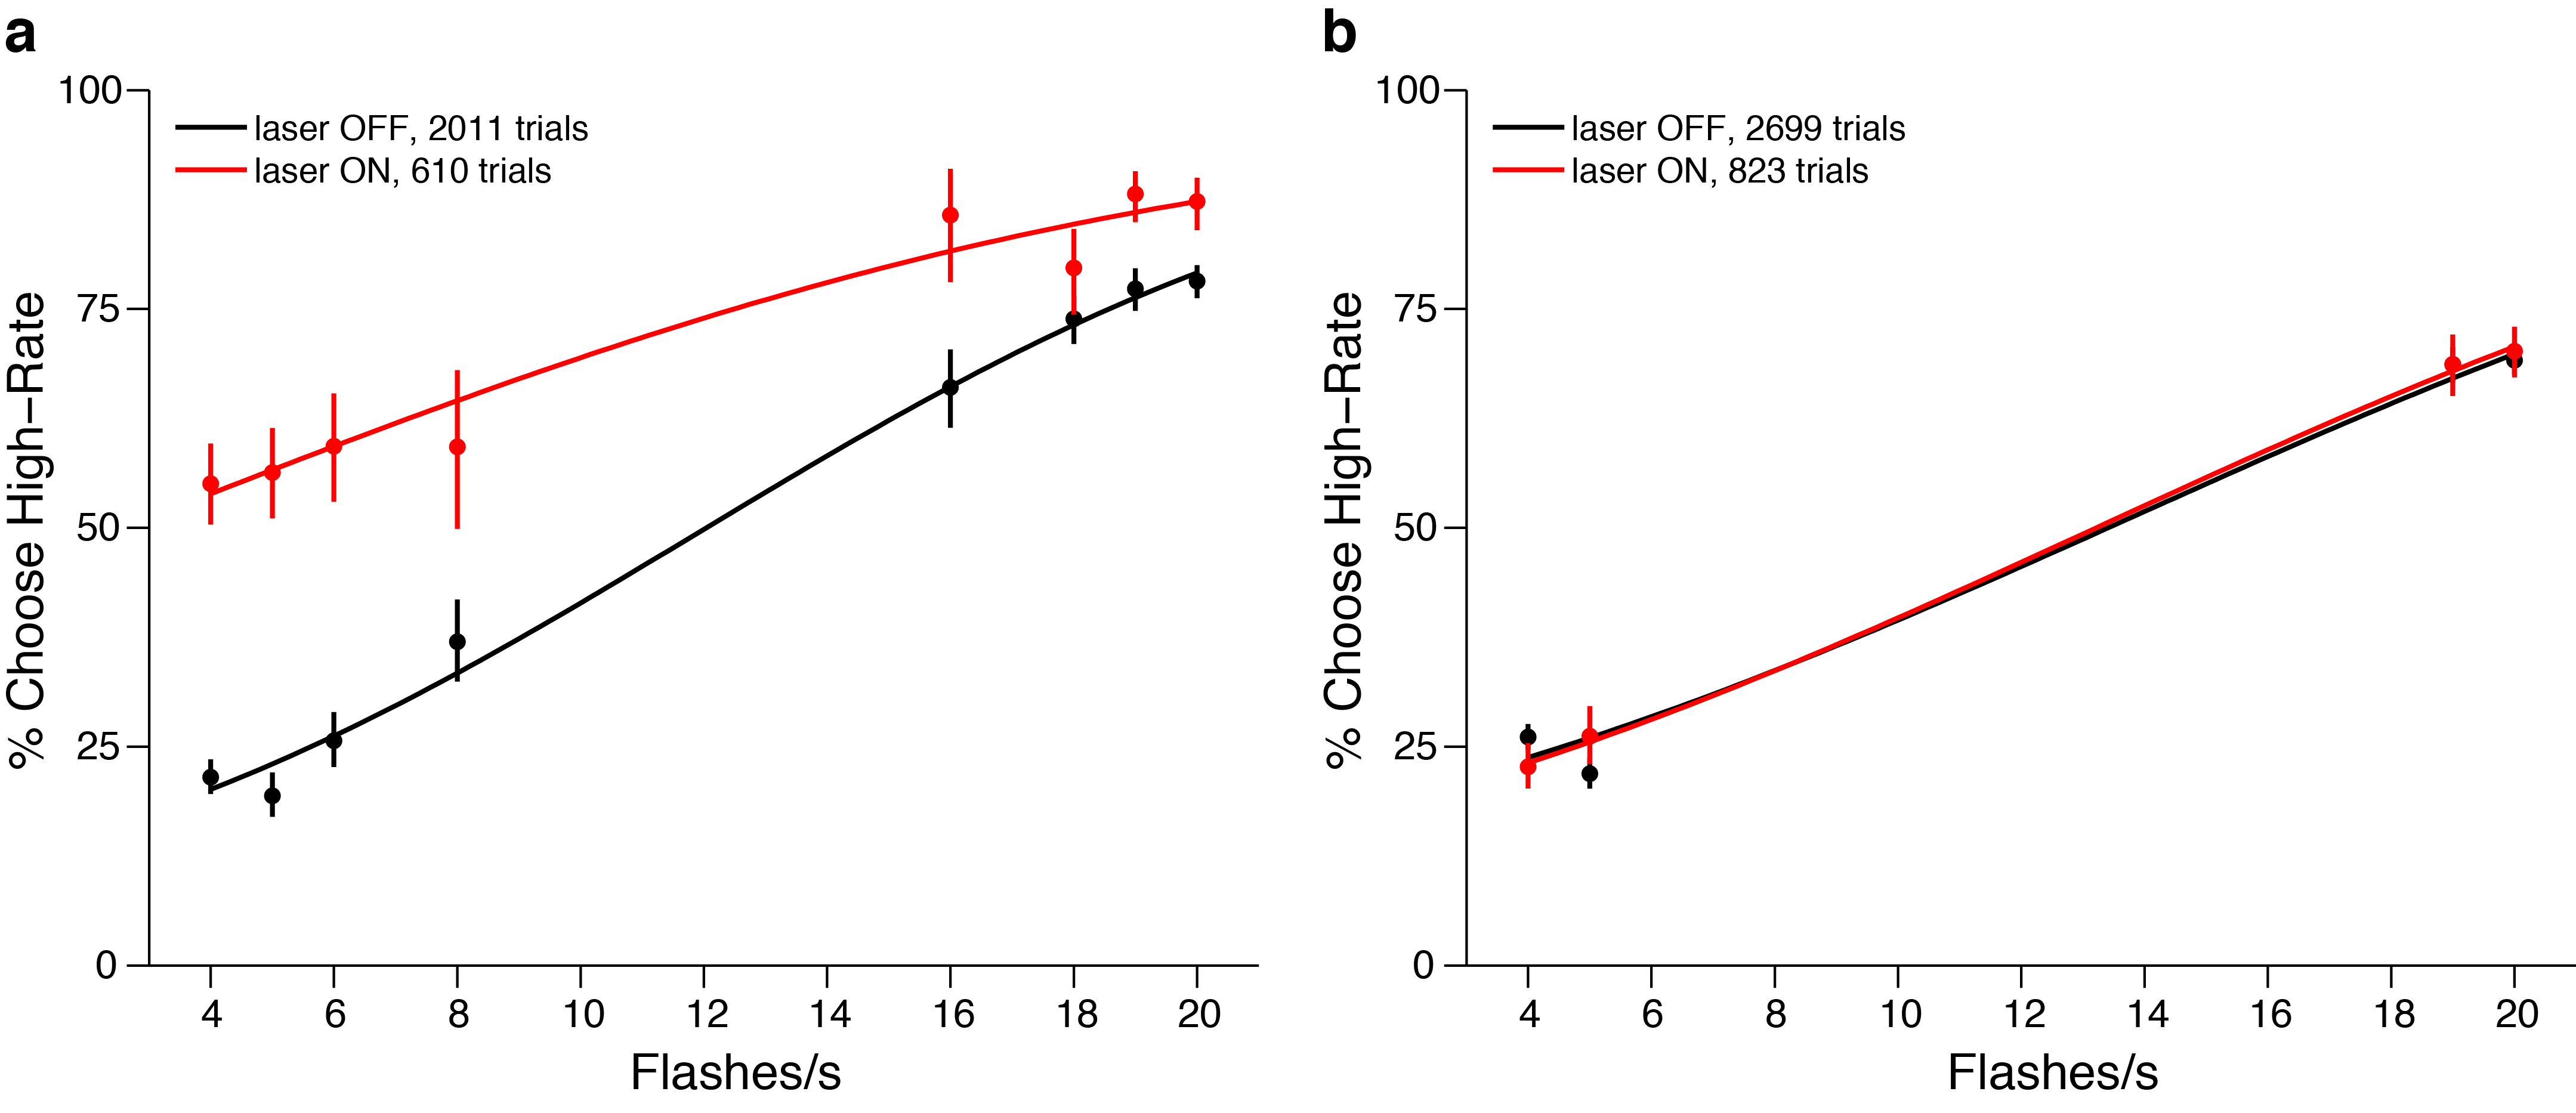
\includegraphics[width=\textwidth]{Figures/chapter4/jaws_controls_summaryPMFs.png}
  \caption[Control Group Summary Psychophysical Data ]{\textbf{Control Group Summary Psychophysical Data} (a) Under identical conditions as Group 1 (ie. no masking red light). Irradiance at 32mW/mm$^{2}$. (b) Masking red light installed in the behavior booth. Irradiance at 64mW/mm$^{2}$. Circles represent the subject's behavioral response during laser OFF (black) and laser ON (red) trials. Solid line represents the psychometric function fit to cumulative Normal (Equation \ref{eq:normalpmf}). Error bars represent Wilson Binomial (95\%) confidence intervals. }
   \label{fig:ctrlsummary}
\end{figure}

\begin{figure}
  \centering
   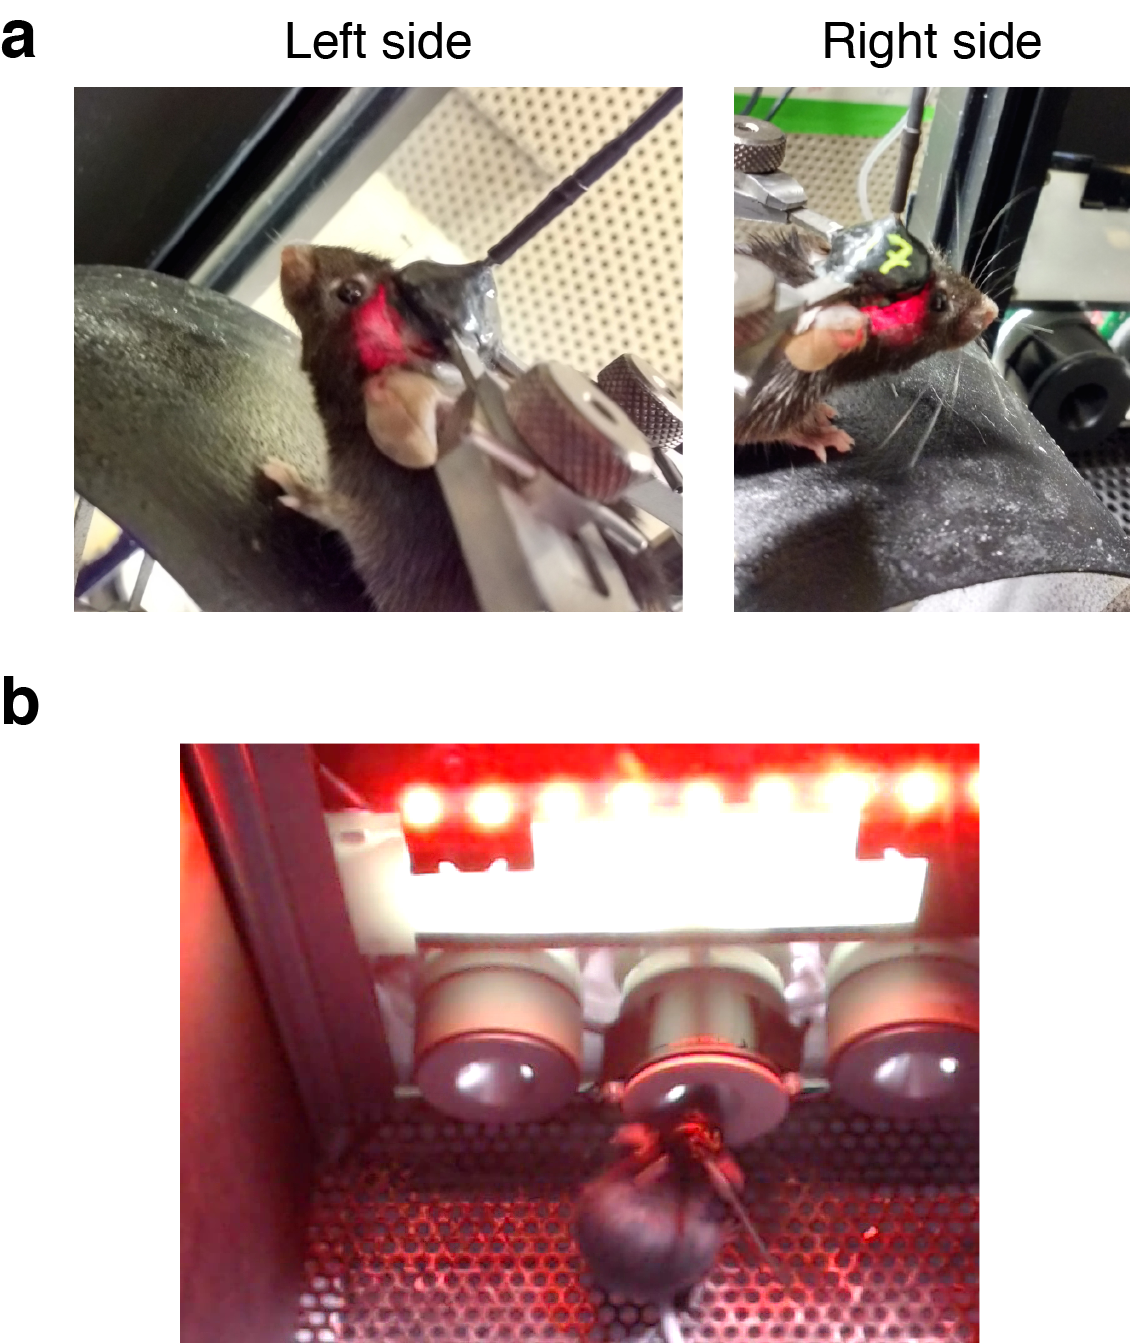
\includegraphics[width=\textwidth]{Figures/chapter4/mouse_house_red_light.png}
  \caption[\emph{In Vivo} Red Light Stimulation and House Red Lights]{\textbf{\emph{In Vivo} Red Light Stimulation and House Red Lights} (a) Left and right side view of mouse implanted with optical fiber with red light \emph{in vivo} illumination at irradiance of 32mW/mm$^{2}$. (b) Mouse in booth with house (masking) red light.}
   \label{fig:mousehouselight}
\end{figure}
%-----------------------------------------------------------------------------
%-----------------------------------------------------------------------------
\subsection{Area AM Inhibition - Group 2}
To distinguish whether the behavioral effects observed in Group 1 (Figure \ref{fig:AMgroup1summary}) were due to a sensory stimulus or spatial/motor bias, and to reduce the artifact caused by \emph{in vivo} red light stimulation, I repeated the area AM inhibition experiments in a new cohort of animals (n = 8 animals, Ai93;ttA;Emx-cre). The cohort of mice (Group 2) were injected with Jaws and implanted with an optical fiber in visual area AM on the left hemisphere. For behavior, they were split into two groups with one group (2A) running on the standard contingency (High-Rate, go RIGHT; Figure \ref{fig:AMgroup2schem} a) and the second group (2B) running on the reverse contingency (High-Rate, go LEFT; Figure \ref{fig:AMgroup2schem}b). Both groups of mice performed the task with the masking red lights to reduce the red light artifact.\par

The results from these two groups of mice make testable predictions that would disentangle whether the observed bias behavioral impact of area AM photoinhibition is sensory or spatial-motor in nature. For example, in the standard behavioral contingency, if the effect of AM photoinhibition is a sensory bias, then inhibition of area AM in both groups should cause a leftward shift in the psychometric function to indicate a bias towards the high-rate port. This would imply opposing spatial motor biases, where Group 2A would exhibit a contralateral bias away from and Group 2B an ipsilateral bias towards the implanted site. However, if inhibition of area AM causes a spatial (motor) bias towards the ipsilateral hemifield, then the psychometric function would shift in the opposing directions for the two groups. Group 2A would exhibit a rightward shift and Group 2B a leftward in the psychometric function. \par 

The psychophysical performance of Group 2 mice was impaired by photoinhibition of area AM (Figure \ref{fig:AMgroup2summary}). Although the behavioral impact on Group 2A and 2B were similar, group 2B (reverse contingency) exhibited pronounced deficits in performance across multiple laser power (irradiance) levels. In Figure \ref{fig:amGLMMparams}a the effect of photoinhibition on the animals' sensitivity ($\beta_{evidence:opto}$) is plotted as function of photoinhibition strength (irradiance, mW/mm$^{2}$). Photoinhibition significantly reduced the slope of the psychometric functions for subjects in Group 2B at irradiance levels 32 mW/mm$^{2}$ (p = 7.2e$^{-05}$) and 64 mW/mm$^{2}$ (p = 3.4e$^{-06}$). The sensitivity of Group 2A subjects was affected only at 32 mW/mm$^{2}$ (p = 7.3e$^{-06}$). Individual psychometric functions fitted to GLMM are shown in Figures \ref{fig:amGLMM16},\ref{fig:amGLMM32}, and \ref{fig:amGLMM64}. \par 

If the both groups of animals experienced a sensory high-rate bias, then the choice biases of both groups should increase with photoinhibition strength. This relationship was only observed in Group 2B, but not in Group 2A mice (Figure \ref{fig:amGLMMparams}b). \par 

\begin{figure}
  \centering
   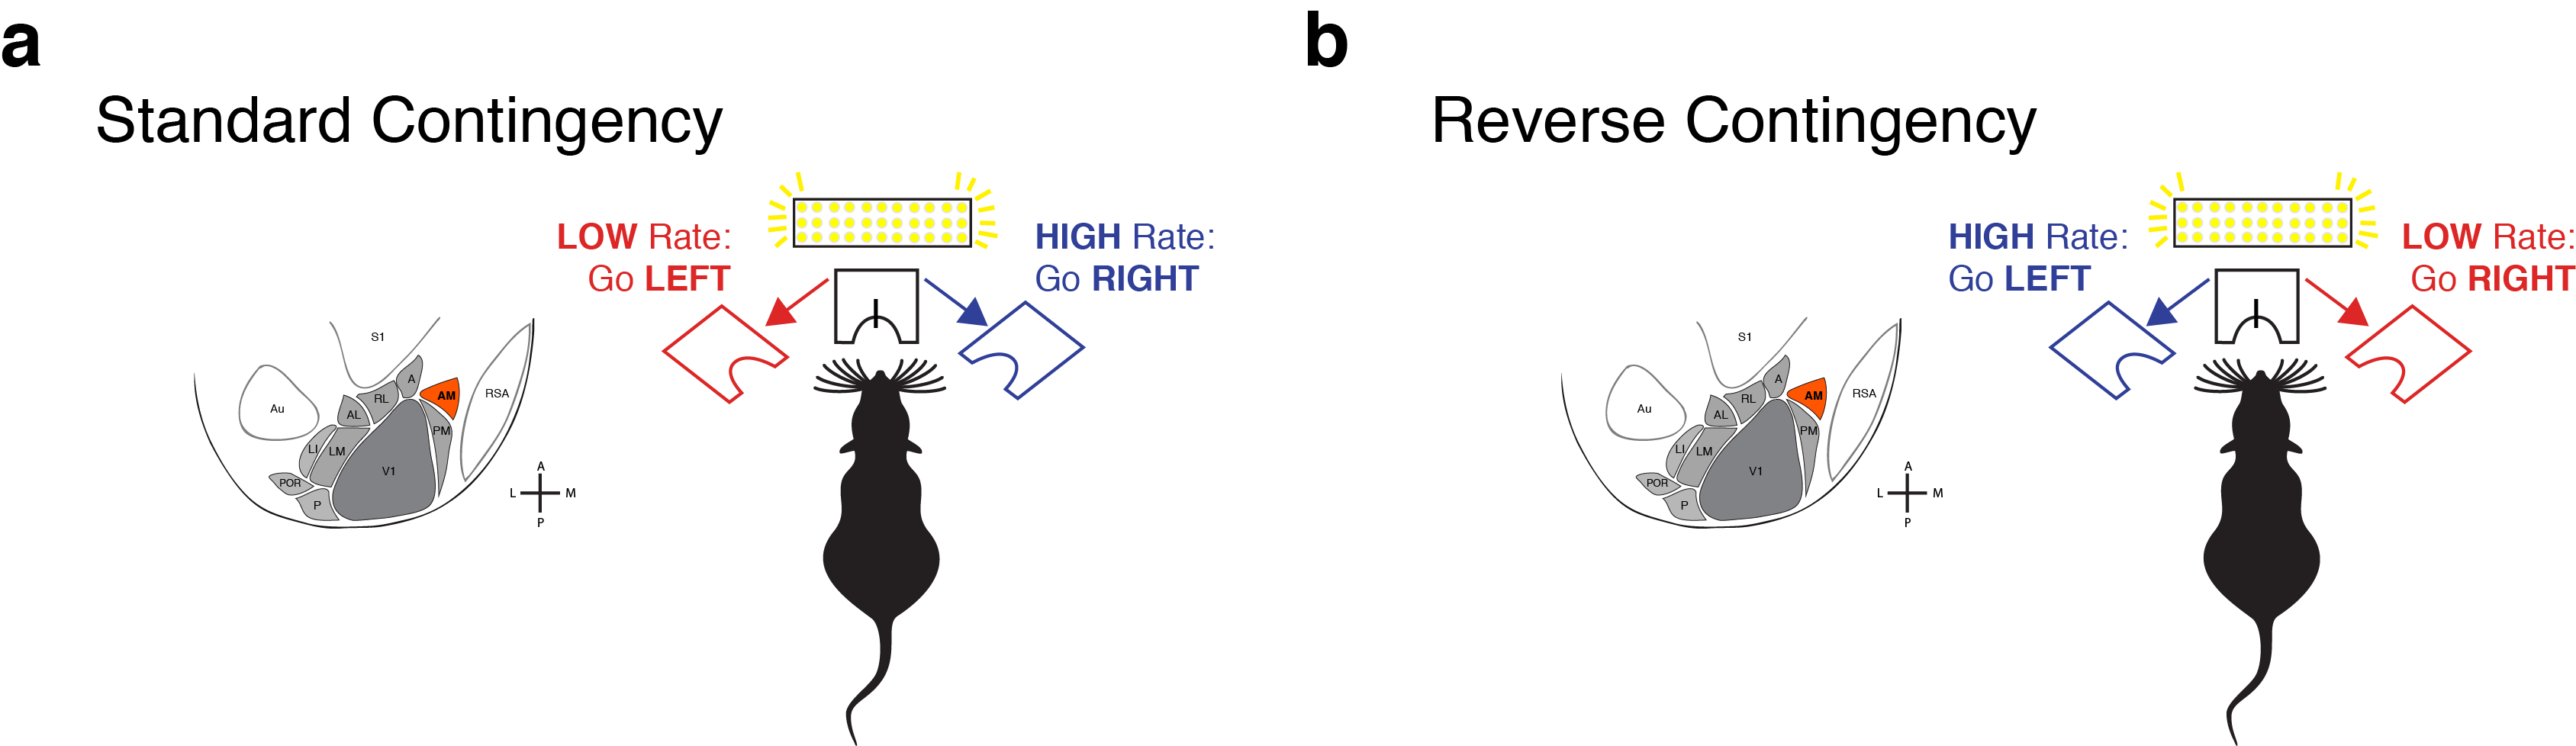
\includegraphics[width=\textwidth]{Figures/chapter4/jaws_AM_group2_schematic.png}
  \caption[Area AM Group 2 Cohort]{\textbf{Area AM Group 2 Cohort} (a) Group A trained on the standard contingency: High-Rate, go RIGHT (b) Group B trained on the reverse contingency: High-Rate, go LEFT. Jaws virus injected in and optical fiber implanted on the left hemisphere.}
   \label{fig:AMgroup2schem}
\end{figure}
%-----------------------------------------------------------------------------
\begin{figure}
  \centering
   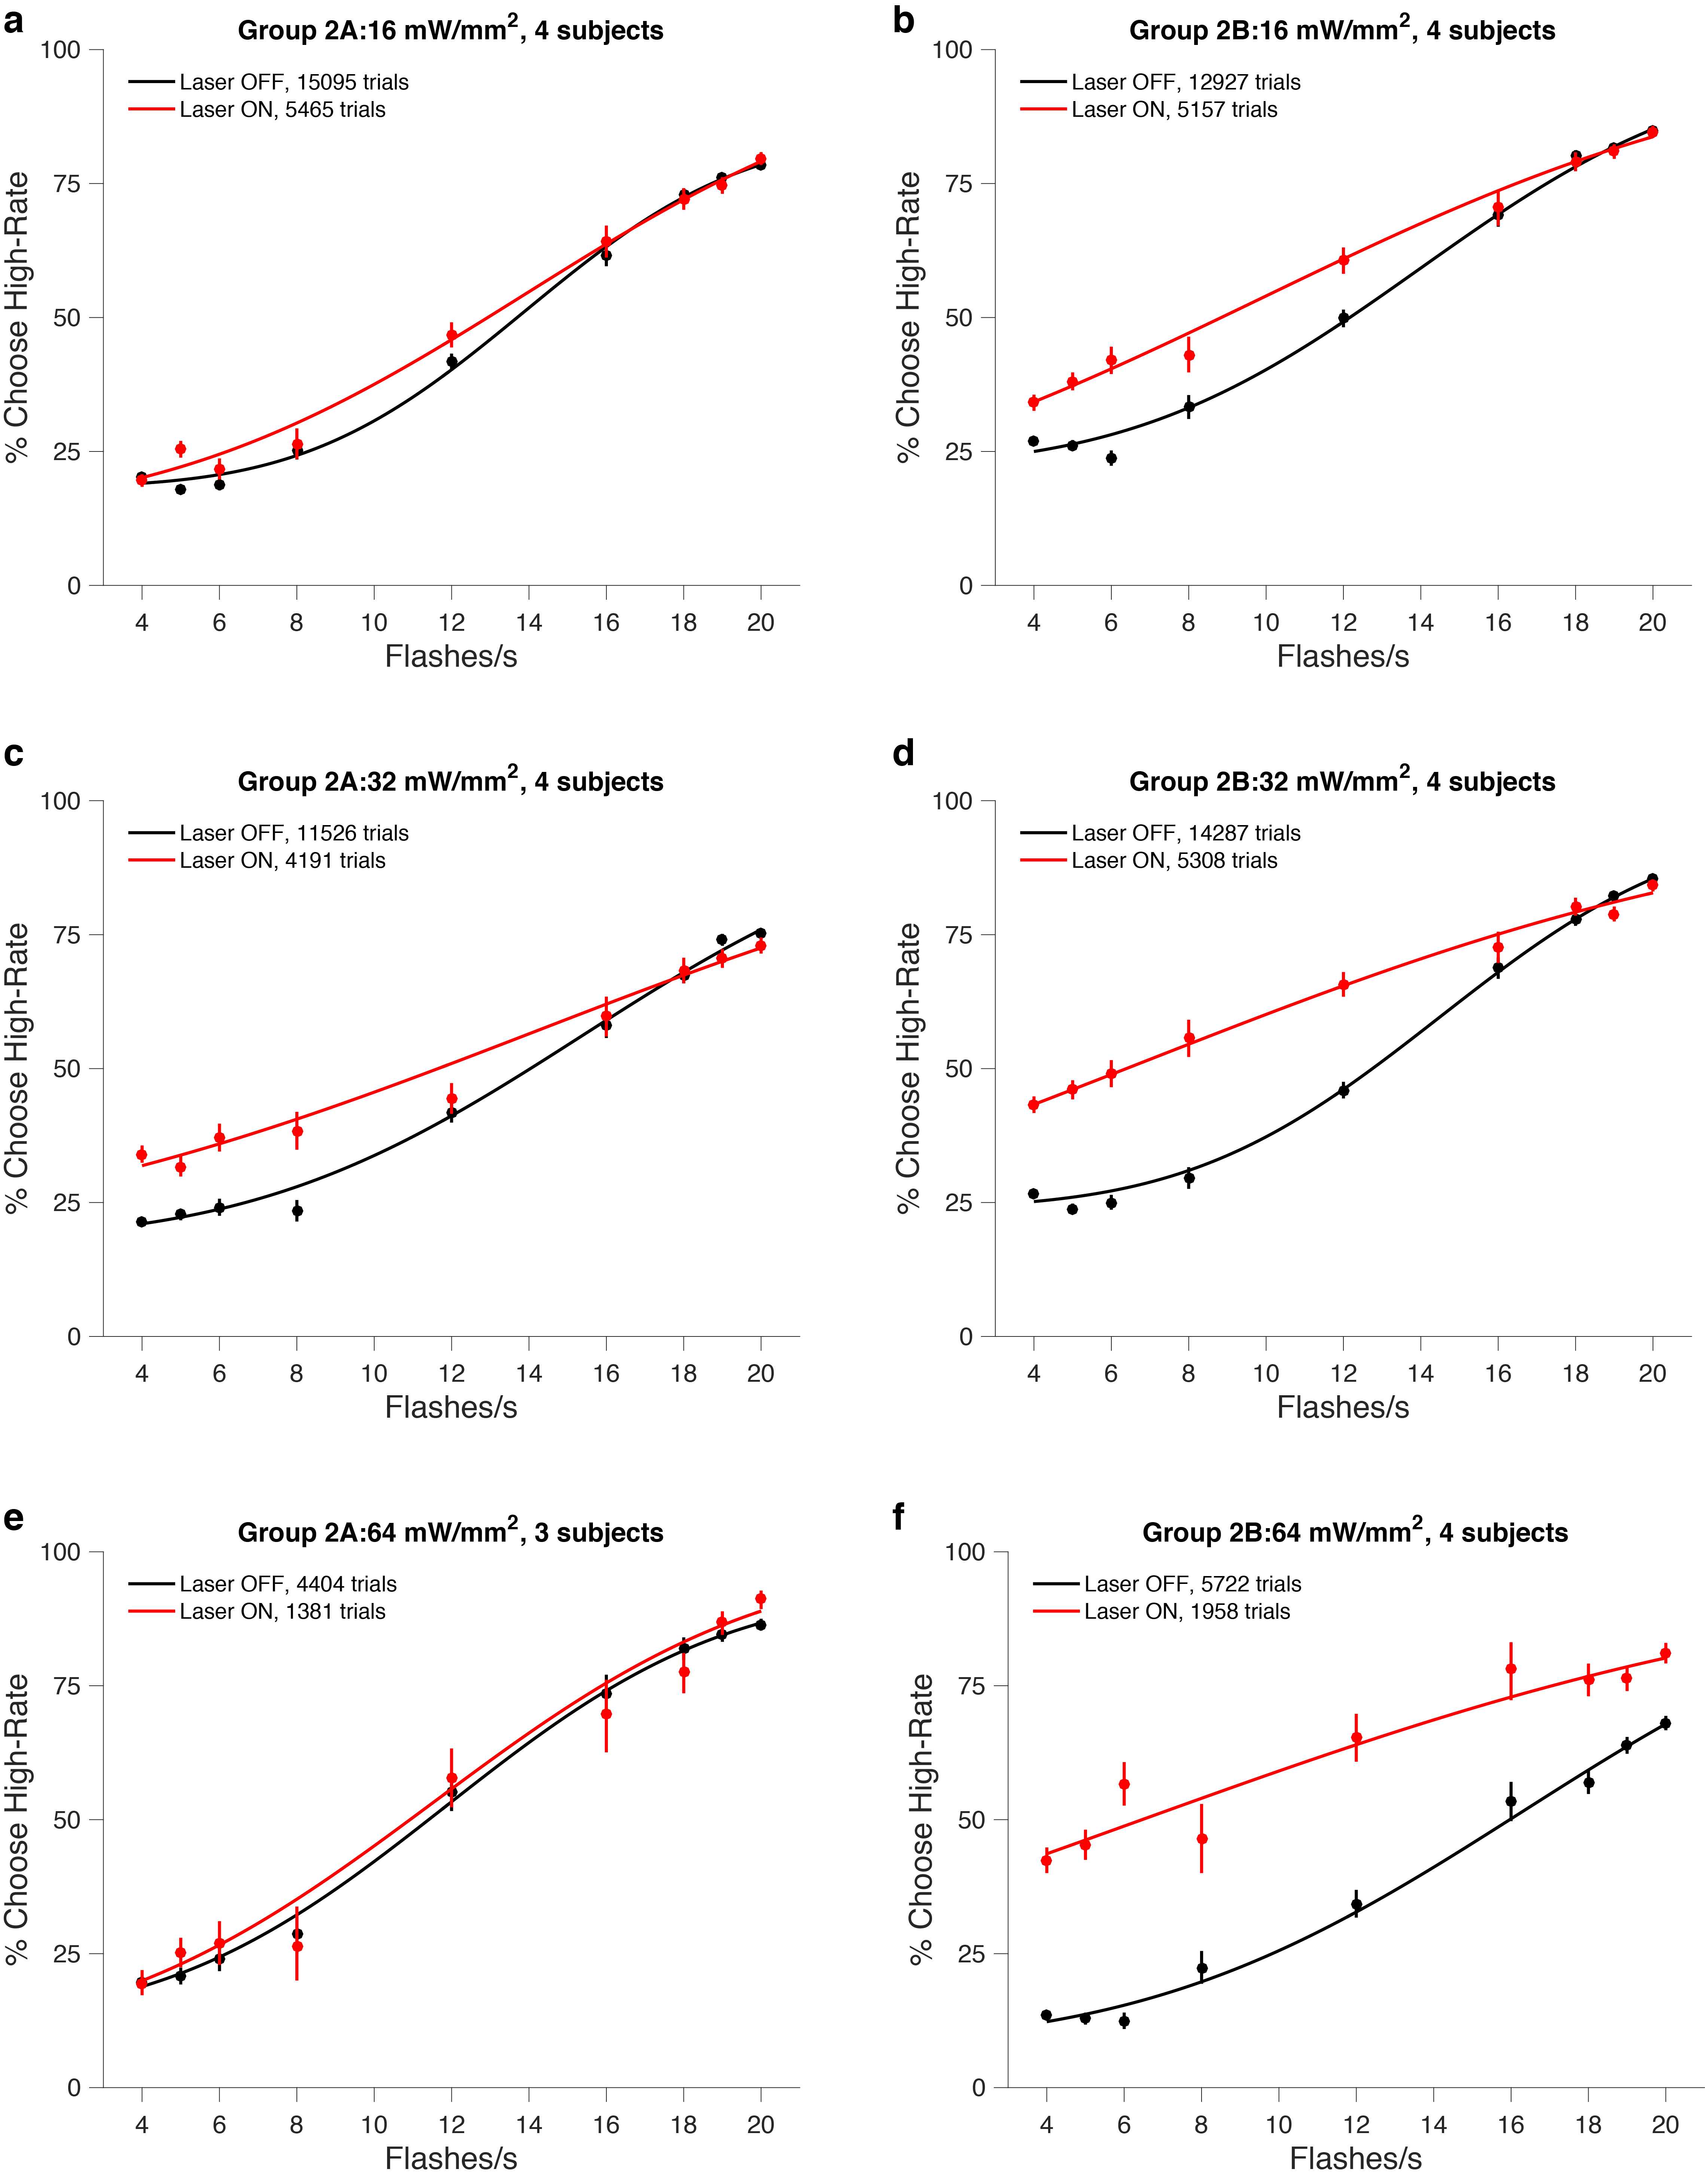
\includegraphics[width=\textwidth,height=0.9\textheight,keepaspectratio]{Figures/chapter4/jaws_AM_group2_summary_PMFs_irradiance.png}
  \caption[Area AM Group 2 Psychometric Data]{\textbf{Area AM Group 2 Psychometric Data} Pooled psychometric function at different irradiance levels for (a,c,e) Group 2A, standard contingency and (b,d,f) Group 2B, reverse contingency. Circles represent psychometric performance at each event rate and the solid line is the psychometric function fit with a cumulative Normal (Equation \ref{eq:normalpmf}). Errors bars represent Wilson binomial confidence intervals on the psychometric data.}
   \label{fig:AMgroup2summary}
\end{figure}
%-----------------------------------------------------------------------------
\begin{figure}
  \centering
   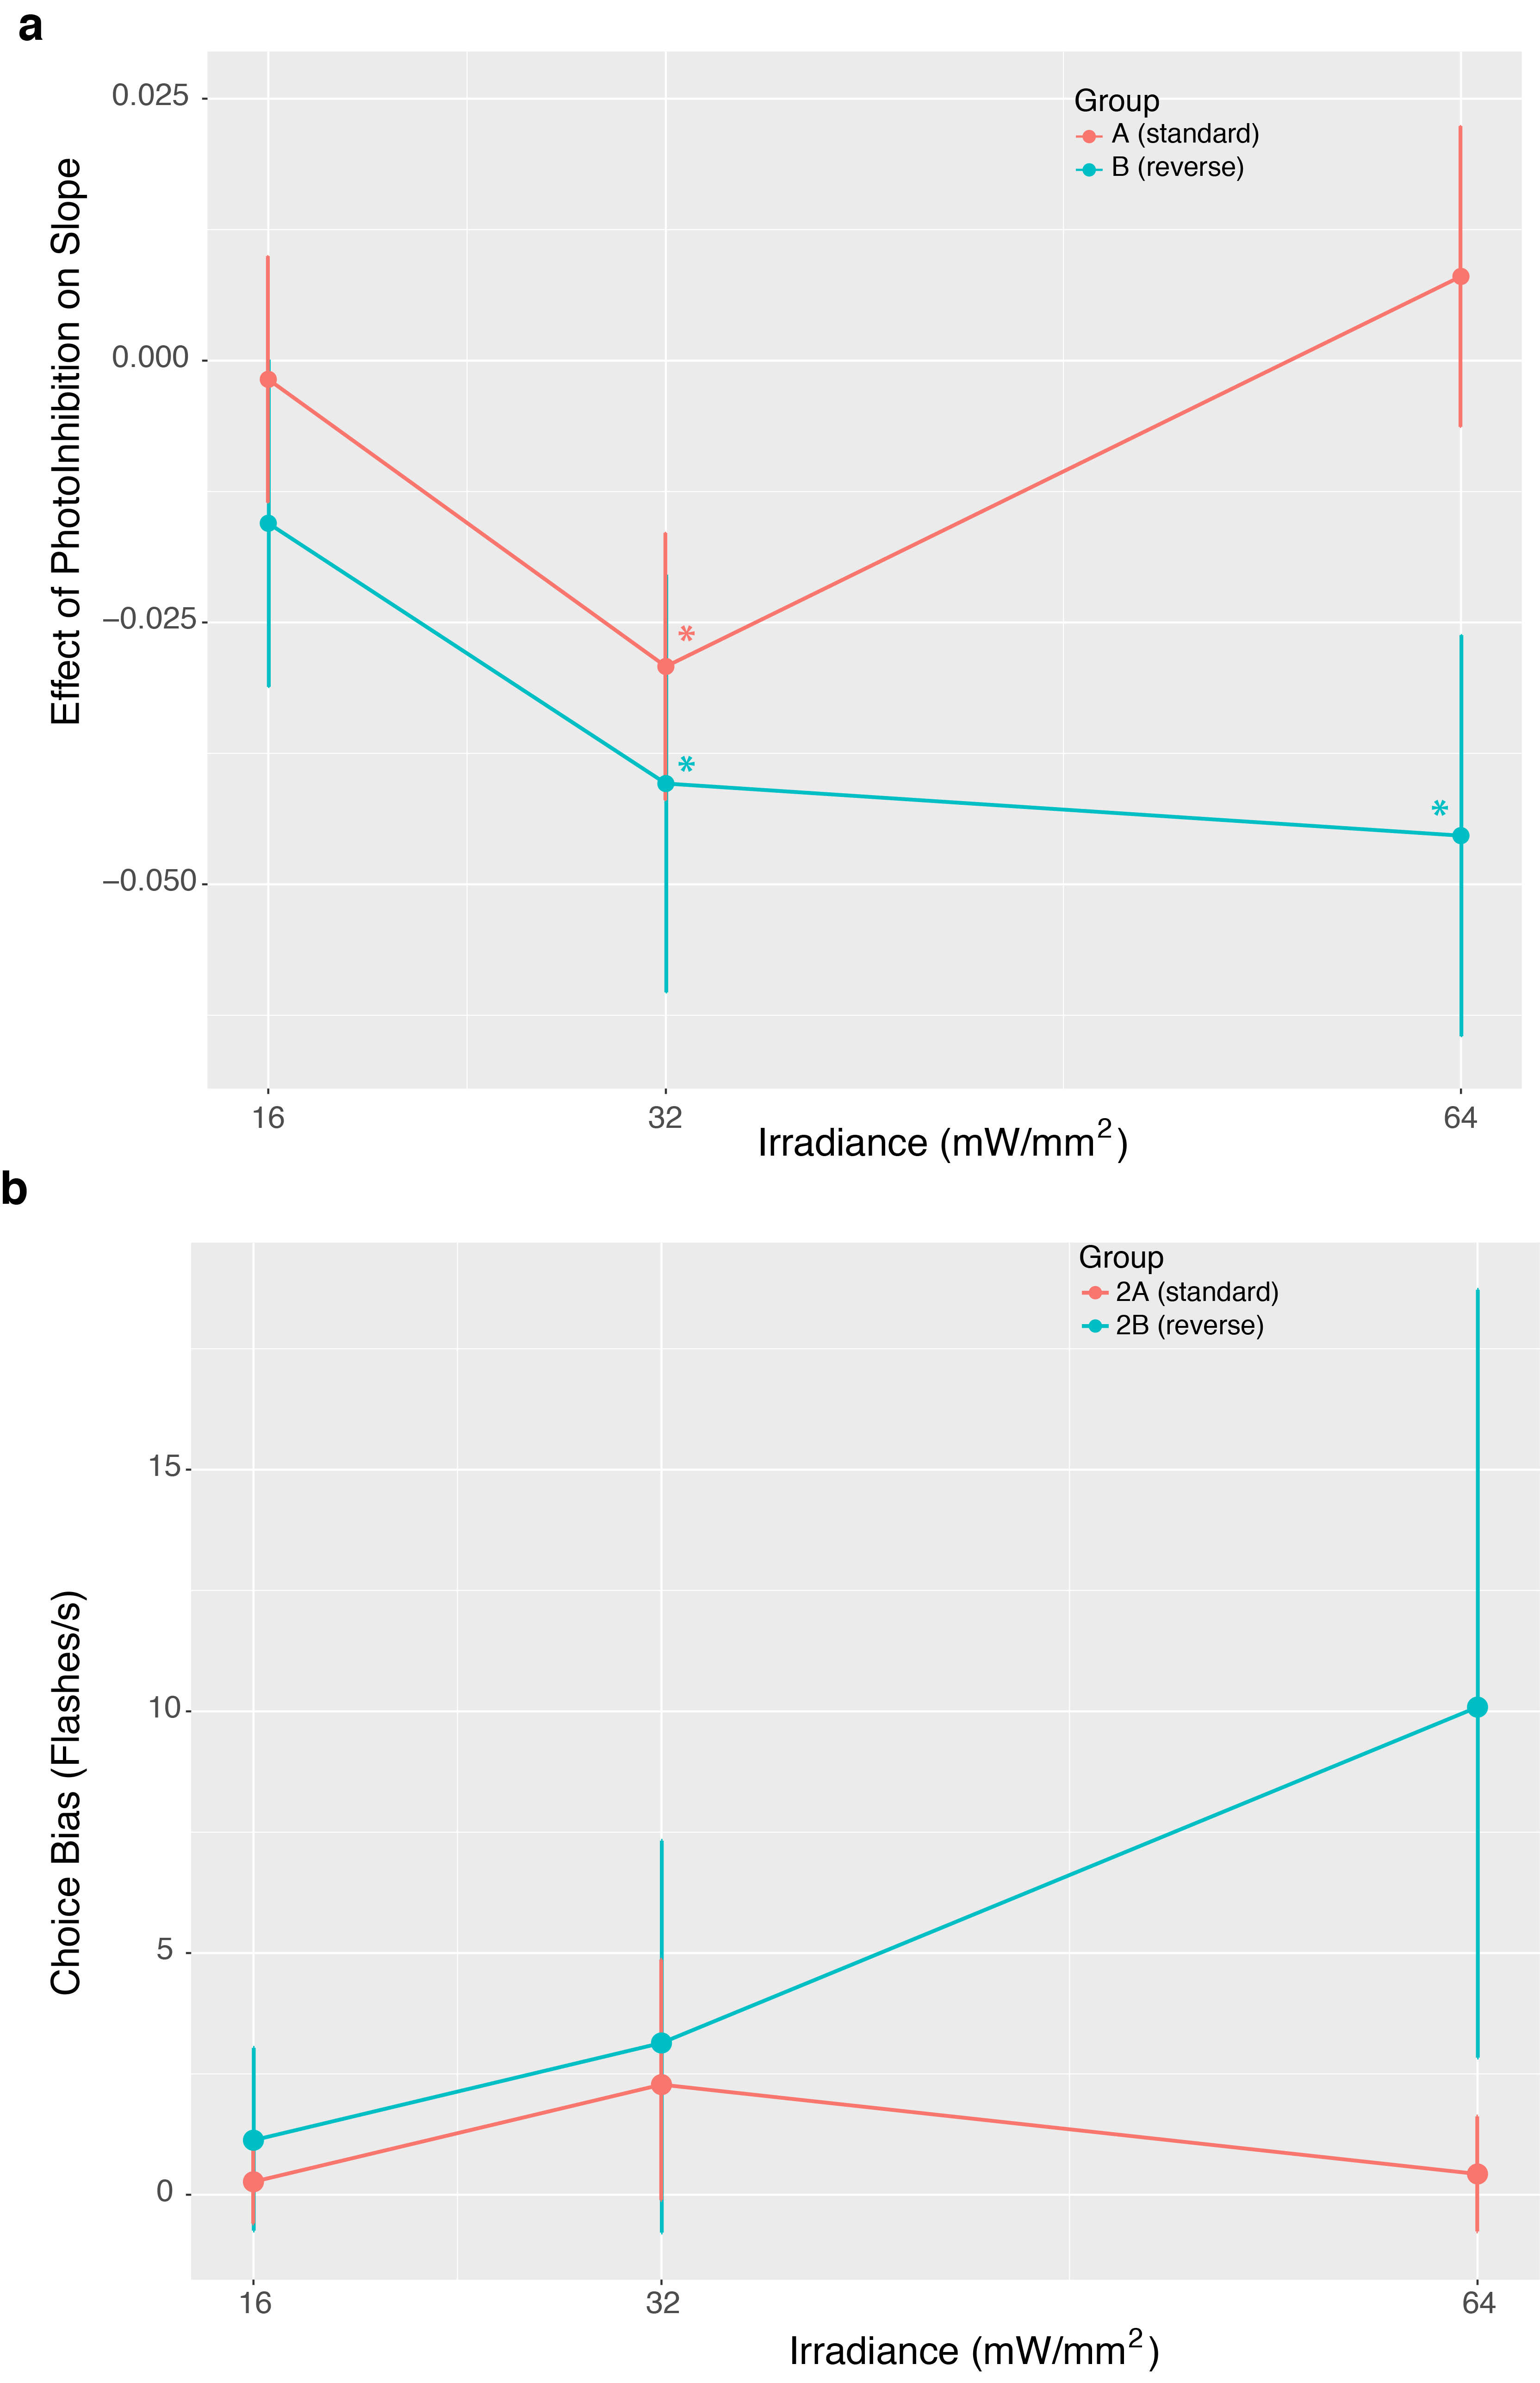
\includegraphics[width=\textwidth,height=0.9\textwidth,keepaspectratio]{Figures/chapter4/glmm_pmf_effects.png}
  \caption[Psychophysical Effects of Area AM Photoinhibition]{\textbf{Psychophysical Effects of Area AM Photoinhibition} Psychophysical parameters estimated from the GLMM model. (a) Effect of area AM photoinhibition on the slope of the psychometric function ($\beta_{evidence:opto}$) as a function of irradiance. Error bars represent 95\% confidence interval. Asterisks mark statistically significant (p<0.05) coefficients. (b) Choice bias as defined in Equation \ref{choicebias}. Choice bias error bars represent 95\% confidence intervals estimated by error propagation. }
   \label{fig:amGLMMparams}
\end{figure}

% %-----------------------------------------------------------------------------
% Figure \ref{fig:highRateBias} summarizes the high-rate bias for each animal. High-rate bias was measured as the difference between percent correct on high-rate choices and low-rate choices. 
% \begin{figure}
%   \centering
%    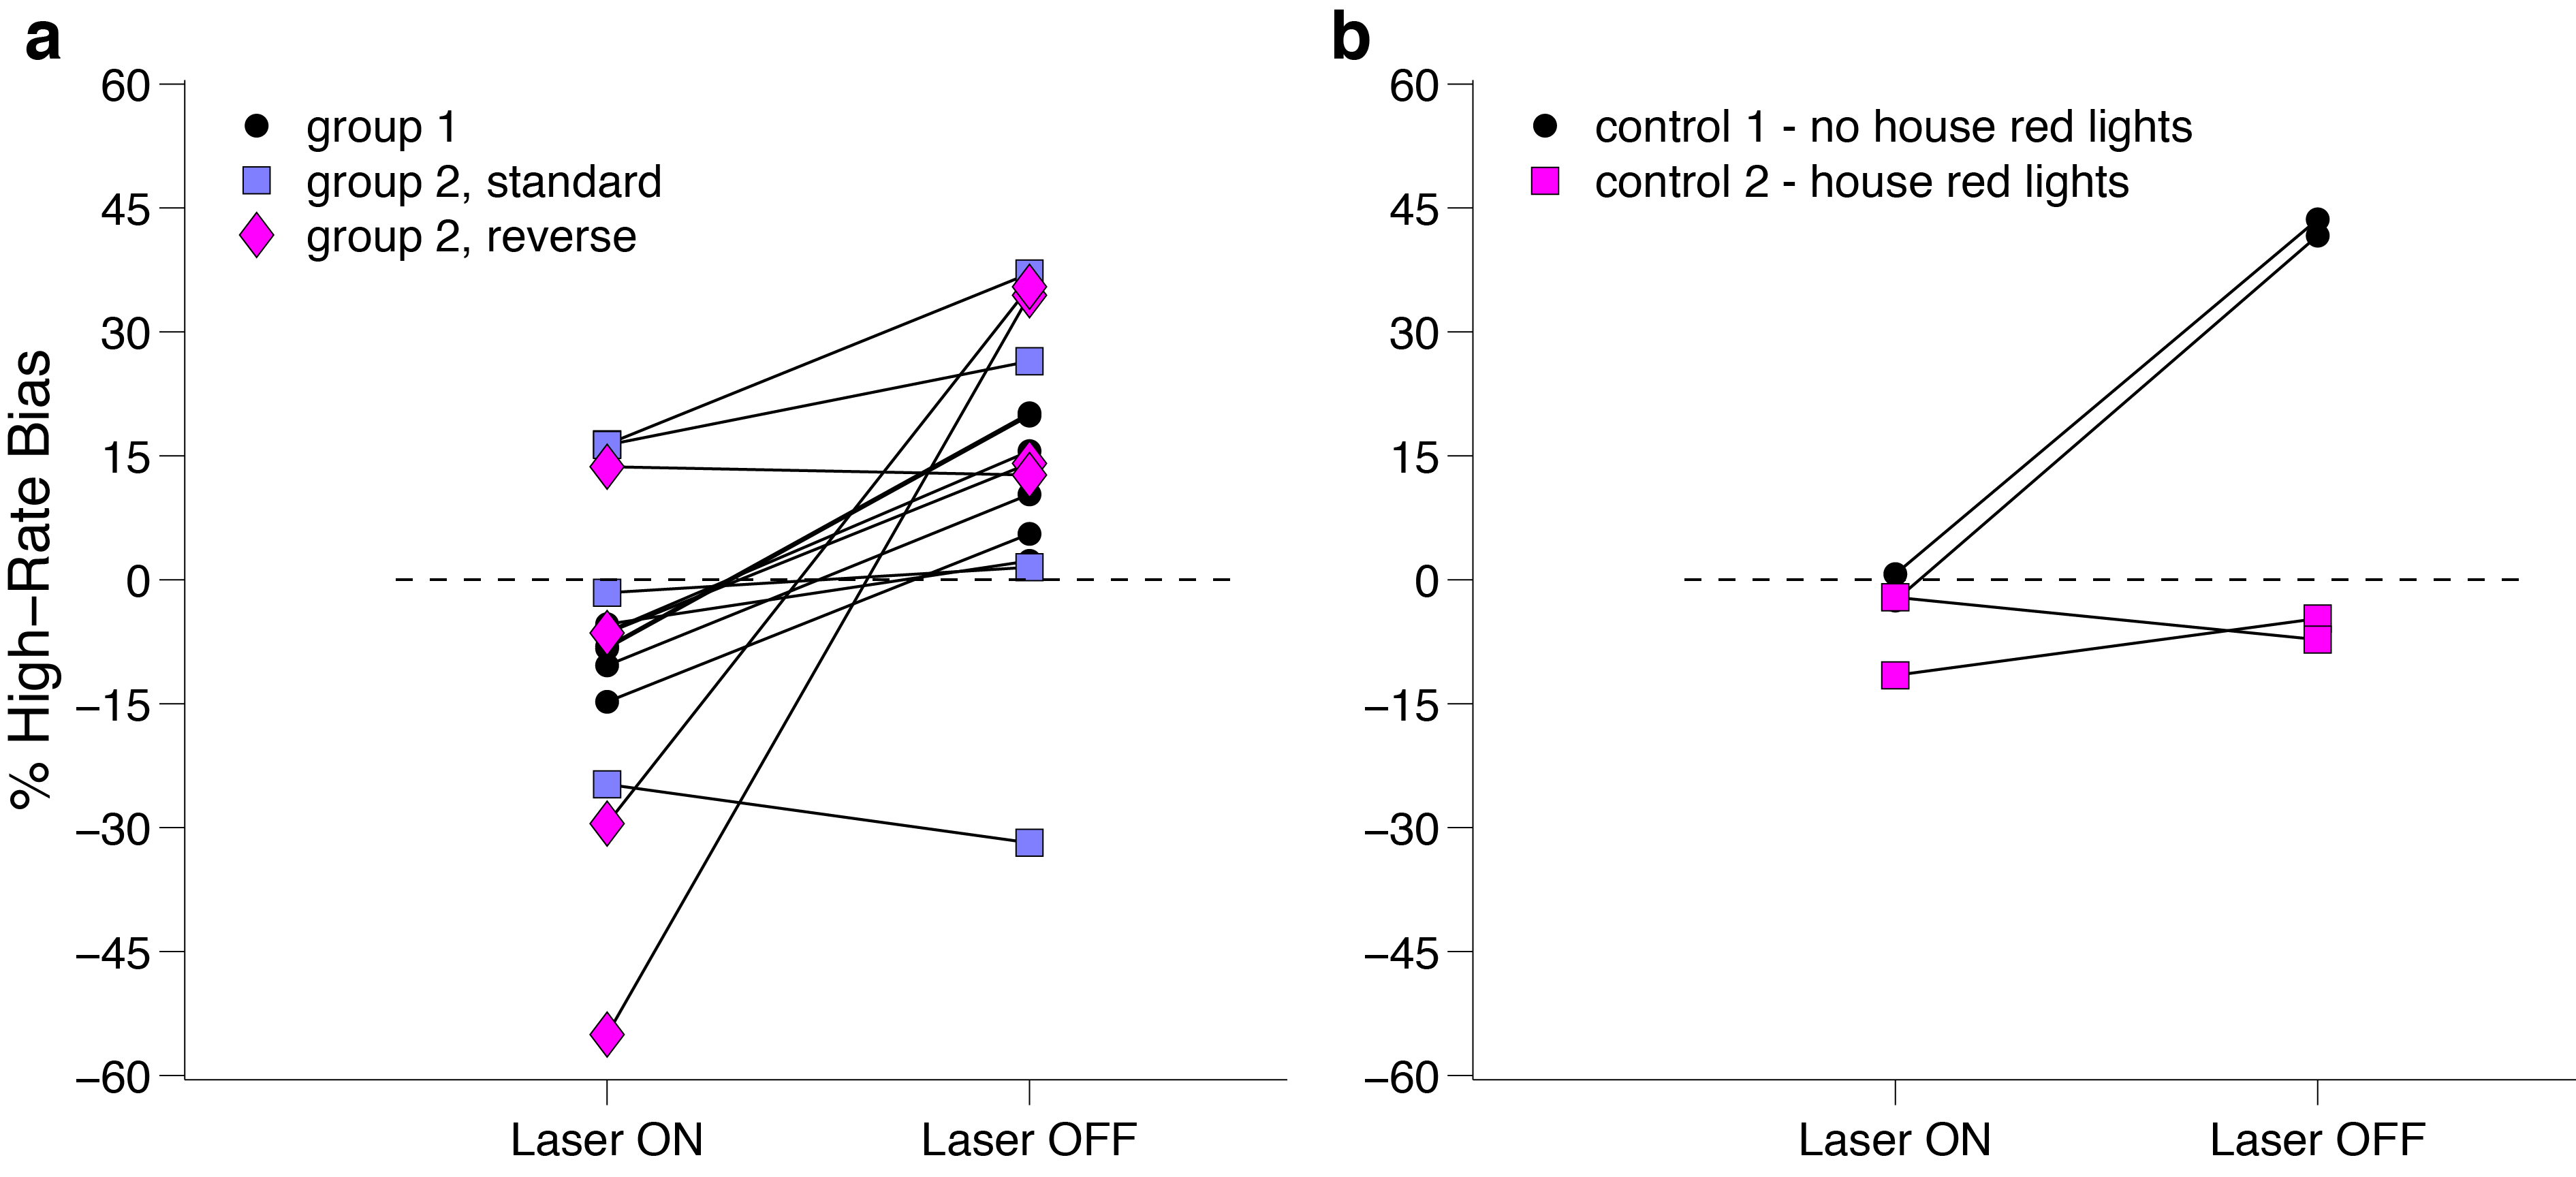
\includegraphics[scale=0.45]{Figures/chapter4/highRateBias.png}
%   \caption[]{\textbf{High-Rate Bias, all mice} }
%    \label{fig:highRateBias}
% \end{figure}
%-----------------------------------------------------------------------------
\section{Discussion}
In this chapter, I presented experiments aimed at silencing mouse secondary visual area AM during visual evidence accumulation. Photoinhibition affected both the sensitivity and choice bias in both groups. However, there were noticeable differences in the effect of photoinhibition. Group 2B mice, implanted on the left hemisphere and trained on the reverse contingency (HIGH-Rate, Go LEFT), were more affected by area AM inhibition in terms of stimulus sensitivity and choice bias (Figure \ref{fig:amGLMMparams}), compared to Group 2A mice trained on the standard contingency. Group 2B mice exhibited a greater tendency to make more high-rate choices during AM photoinhibition, in addition to an ipsilateral bias towards the fiber implanted hemifield. This effect is also consist with that observed in Group 1 mice, who were trained in the absence of the masking red light. \par 

A plausible explanation for the observed differences between the two groups is unilateral photoinhibition of area AM causes a bias towards the ipsilateral hemisphere. However, this effect is combined with the residual high-rate artifact caused by \emph{in vivo} red light stimulation (Figures \ref{fig:ctrlsummary} and \ref{fig:ctrlpmfs}). In Group 2B mice, the photoinhibition site (located on the left hemisphere) and high-rate (left hemifield) choice port are congruent, hence upon photoinhibition the effect area AM photoinhibition and the red light artifact sum together to produce the apparent high-rate bias. On the other hand, in Group 2A mice, the photoinhibition site (left hemisphere) and high-rate choice port (right hemifield) are incongruent; hence, the effect of area AM inhibition and the red light artifact would compete, and in some regimes cancel each other. Consistent with this hypothesis, at 64 mW/mm$^{2}$ photoinhibition Group 2A mice exhibit no change in choice bias or the sensitivity. However at 32 mW/mm$^{2}$ the choice bias tends toward positive, and may be a result of the residual red light artifact which is greater than the proposed ipsilateral bias effect caused by area AM inhibition. \par

The confound introduced by the red light source used for photoinhibition makes it difficult to disentangle the true nature of the effect of area AM photoinhibition. The artifact was greatly reduced (Figure \ref{fig:glmmcontrol}), although not eliminated, by training the mice with house red lights (Figure \ref{fig:ctrlpmfs}). The artifact is most likely caused by red light propagating from the stimulation site and directly activating the retina from within \parencite{Danskin2015} and producing an apparent increase in overall brightness, which is correlated with the high-rate flashes (Figure \ref{fig:brightnessSim}). \textcite{Danskin2015} measured retinal activation during \emph{in vivo} red light stimulation and found the largest activation ipsilateral to the implanted stimulation fiber. This would imply that mice would have an increased tendency to go towards the hemifield ipsilateral to the implanted fiber. Since the visual pulses stimuli is non-spatial it is unlikely that the mice are directly biased towards the implant site. Instead, the behavioral artifact of red light stimulation might arise if the mice were using perceived brightness over time as a strategy to solve the visual pulses task. The nature of the visual pulses stimulus is such that the average brightness (or amount of photons) over time is correlated with the number of flashes (Figure \ref{fig:brightnessSim}). The high-rate stimulus is the stimulus that is also the brightest or emits the most number of photons over time and conversely the low-rate stimulus emits the least number of photons over time. Hence, during \emph{in vivo} red light stimulation, the light escaping the eyes combines with the incoming light from the visual pulses stimuli and increases the perceived brightness (Figure \ref{fig:brightnessSim}b). This may cause the animal to make a high-rate choice. Brightness manipulation experiments on the visual pulses task (Chapter \ref{Chapter2}) suggests that the psychophysical performance of the mice is not entirely invariant to changes in the brightness of the flashes, and that mice may be using a combination of individual flash counting and perceived brightness over time to solve the task.\par 
%-----------------------------------------------------------------------------
\begin{figure}
  \centering
   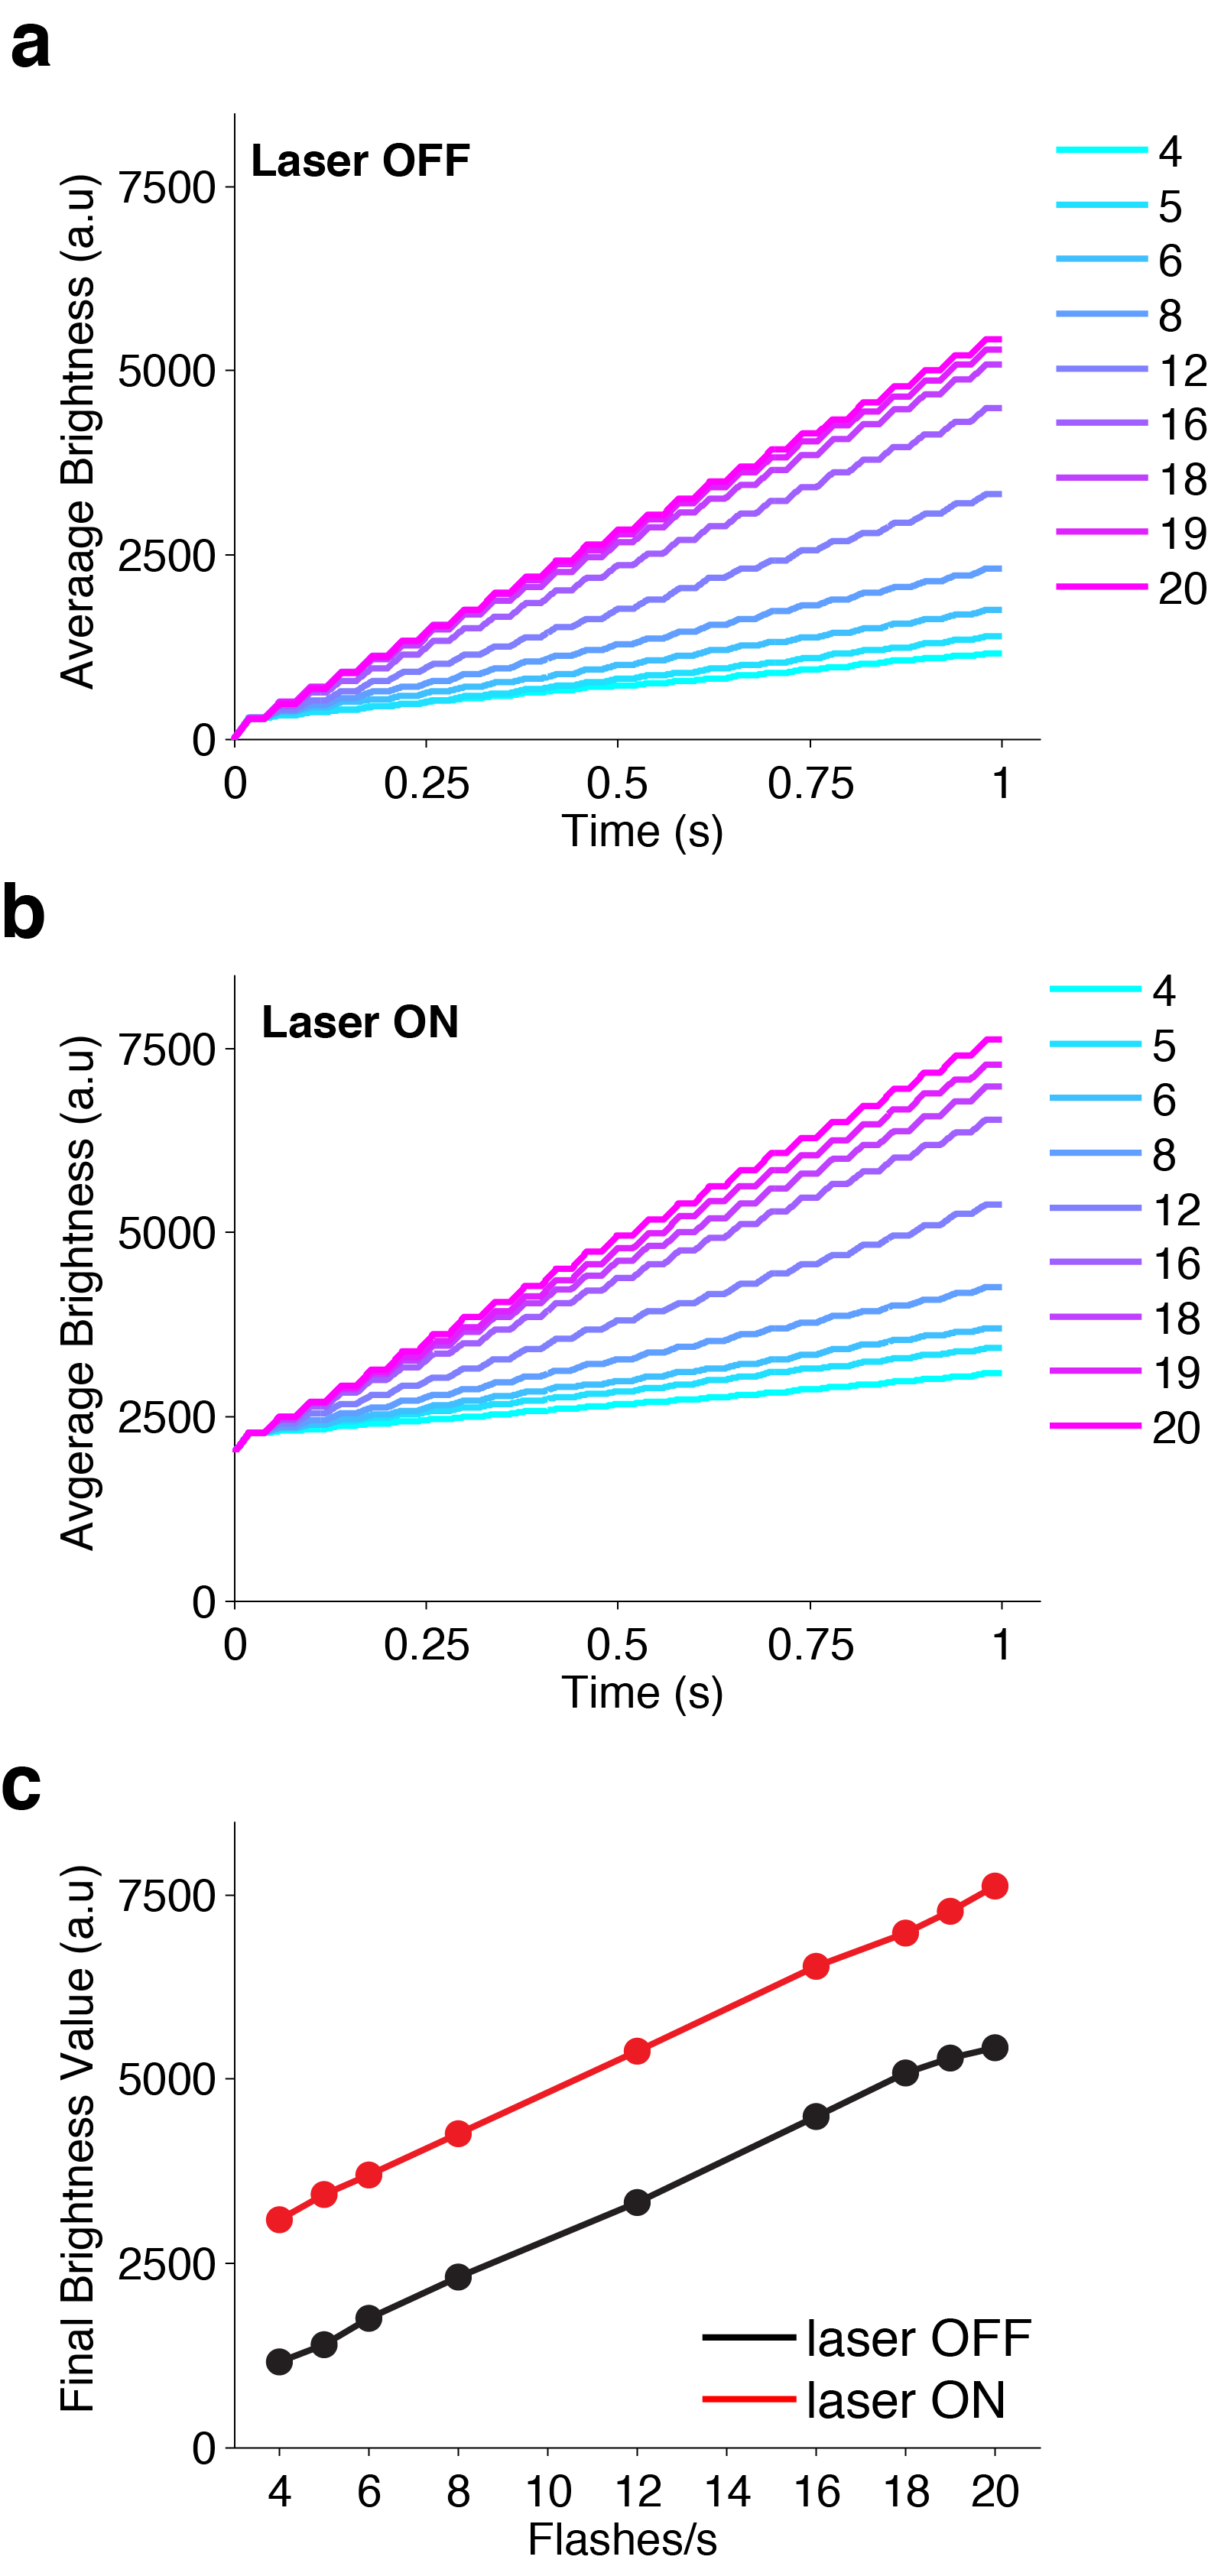
\includegraphics[width=\textwidth,height=0.9\textheight,keepaspectratio]{Figures/chapter4/brightnes_simulation_opto.png}
  \caption[Schematic of Simulated Average Apparent Brightness Over Time]{\textbf{Schematic of Simulated Average Apparent Brightness Over Time} (a) for laser off and (b) laser on condition.(c) The final value from Figure \ref{fig:brightnessSim} plotted against the number of flashes per second for laser OFF (black) and laser ON (red) conditions.}
   \label{fig:brightnessSim}
\end{figure}
%-----------------------------------------------------------------------------
%-----------------------------------------------------------------------------

\begin{table}
\centering
\resizebox{\textwidth}{!}{%
\begin{tabular}{@{}cccccccc@{}}
\toprule
\textbf{Group} & \textbf{\begin{tabular}[c]{@{}c@{}}Sample\\ Size\end{tabular}} & \textbf{\begin{tabular}[c]{@{}c@{}}Implant\\  Side\end{tabular}} & \textbf{\begin{tabular}[c]{@{}c@{}}High-Rate \\ Side\end{tabular}} & \textbf{\begin{tabular}[c]{@{}c@{}}Masking\\ Light\end{tabular}} & \textbf{\begin{tabular}[c]{@{}c@{}}Irradiance\\ (mW/mm\textasciicircum 2)\end{tabular}} & \textbf{\begin{tabular}[c]{@{}c@{}}Interaction\\ b\_evid:opto\end{tabular}} & \textbf{\begin{tabular}[c]{@{}c@{}}Choice Bias\\ (Flashes/s)\end{tabular}} \\ \midrule
\textbf{1} & 6 & R & R & No & 32 & \begin{tabular}[c]{@{}c@{}}-0.021*\\ {[}-0.034   -0.0085{]}\end{tabular} & \begin{tabular}[c]{@{}c@{}}3.47\\ {[}2.46   4.54{]}\end{tabular} \\
\textbf{Control} & 2 & R & R & No & 32 & \begin{tabular}[c]{@{}c@{}}-0.038*\\ {[}-0.056  -0.020{]}\end{tabular} & \begin{tabular}[c]{@{}c@{}}9.72\\ {[}6.3   13.60{]}\end{tabular} \\
\textbf{} &  &  &  & Yes & 64 & \begin{tabular}[c]{@{}c@{}}-0.026*\\ {[}-0.044 -0.0085{]}\end{tabular} & \begin{tabular}[c]{@{}c@{}}2.244\\ {[}0.49   4.37{]}\end{tabular} \\
\textbf{2A} & 4 & L & R & Yes & 16 & \begin{tabular}[c]{@{}c@{}}-0.0018\\ {[}-0.014   9.97e-03{]}\end{tabular} & \begin{tabular}[c]{@{}c@{}}0.27\\ {[}-0.60  1.14{]}\end{tabular} \\
\textbf{} &  &  &  & Yes & 32 & \begin{tabular}[c]{@{}c@{}}-0.029*\\ {[}-0.042   -1.64e-02{]}\end{tabular} & \begin{tabular}[c]{@{}c@{}}2.28\\ {[}-0.092  4.84{]}\end{tabular} \\
\textbf{} &  &  &  & Yes & 64 & \begin{tabular}[c]{@{}c@{}}0.008\\ {[}-0.0063   2.24e02{]}\end{tabular} & \begin{tabular}[c]{@{}c@{}}0.43\\ {[}-0.75  1.62{]}\end{tabular} \\
\textbf{2B} & 4 & L & L & Yes & 16 & \begin{tabular}[c]{@{}c@{}}-0.016\\ {[}-0.031   8.83e-05{]}\end{tabular} & \begin{tabular}[c]{@{}c@{}}1.13\\ {[}-0.76  3.045{]}\end{tabular} \\
\textbf{} &  &  &  & Yes & 32 & \begin{tabular}[c]{@{}c@{}}-0.040*\\ {[}-0.06   -2.2e-02{]}\end{tabular} & \begin{tabular}[c]{@{}c@{}}3.14\\ {[}-0.75  7.28{]}\end{tabular} \\
\textbf{} &  &  &  & Yes & 64 & \begin{tabular}[c]{@{}c@{}}-0.045*\\ {[}-0.064   -2.62e-02{]}\end{tabular} & \begin{tabular}[c]{@{}c@{}}10.09\\ {[}2.84  18.72{]}\end{tabular} \\ \bottomrule
\end{tabular}%
}
\caption[GLMM Analysis Summary Table]{\textbf{GLMM Analysis Summary Table}. * statistically significant coefficients (p < 0.05) }
\label{table:glmm}
\end{table}
%-----------------------------------------------------------------------------%-----------------------------------------------------------------------------

The proposed ipsilateral bias caused by AM photoinhibition is consistent with spatial hemineglect observed in visual parietal lesions. Spatial hemineglect, also referred to as contralateral neglect, is a phenomenon that occurs when subjects ignore the contralateral hemifield as a result of lesion to the parietal cortex. Although hemineglect has been observed in humans \parencite{Stone1991,Kerkho2001} and rats \parencite{Crowne1986,Reep2009}, it is not clear whether neglect has been observed in mice. The presence of hemispatial neglect would suggest that the mice are neglecting the tendency to go towards the affected (contralateral) visual hemifield. Therefore, in the presence of a red light artifact, mice trained on opposite behavioral contingencies should yield the same effect, i.e. a bias ipsilateral to the stimulation hemisphere. \par 

Another related, and plausible, interpretation for the ipsilateral bias due to suppression of AM activity is that neurons in AM likely represents the "intent" to make contralateral choices. Intention, in the neuroscience literature, is defined as an early plan for movement, which specifies the goal and type of movement \parencite{Andersen2002}. Under the intention scenario, the two hemispheres of AM would represent competing movement intentions, such that inactivation of one hemisphere leads to movement in the opposing direction. 
%This framework makes an interesting prediction for bilateral inactivation of AM. In this scenario, the psychometric function would appear shallower (Figure \ref{fig:predictions}b) reflecting a loss in sensitivity as contralateral movement intentions on both hemispheres are impaired. \par 

To test the proposed spatial hemineglect (or impaired intent) caused by area AM inhibition, one could train mice on a visual pulses task with two additional interspersed conditions: instructed and free choice \parencite{Erlich2015,Katz2016}. On the instructed trials, the animals are cued to a the reward port by a brief LED flash at the reward port, and in the free choice trials, both LEDs are turned on and the animal can freely choose either reward port to receive the reward. If visual area AM plays a role in spatial neglect (or contralateral movement intent), inactivation should only affect free choice trials and not the instructed trials. Because the animal chooses where to go on the free choice trials, if area AM plays a role in the intent to make contralateral movements, unilateral inactivation of area AM would bias the subject towards the hemifield ipsilateral to the stimulation site.\par 

For this study, Jaws was an attractive inhibitory opsin to use primarily because it outperformed other available inhibitory opsins such as ArchT and Halo in terms of inhibition \parencite{Chuong2014}. Despite the powerful inhibition afforded by Jaws, future studies would benefit from avoiding red light sensitive opsins altogether for experiments in mice performing visually-guided behaviors. Further efforts are needed to carefully characterize available optogenetic inhibitory tools that provide potent inhibition and do not interfere with the behavior. This requirement is dependent on the several factors such as the nature of the task, stimulus, and brain area(s) of interest. Nevertheless, several alternative optogenetic strategies are available, including blue light sensitive anion conducting channelrhodopsin (SwiChR or iC1C2) \parencite{Berndt2014,Berndt2016} or excitation of inhibitory neurons \parencite{Madisen2012,Glickfeld2013b,Poort2015,Burgess2016}. The latter approach presents a technical challenge for working with GCaMP6 transgenic mice, which are typically bred to express GCaMP6 in excitatory neurons \parencite{Madisen2015}. One could produce transgenic mice that express GCaMP6 in the inhibitory neurons (PV+ or Gad2+); however, it is not obvious whether mouse lines expressing GCaMP6 in inhibitory neurons could replicate the retinotopic widefield maps obtained with the existing GCaMP6 mouse lines. A solution that is compatible with the existing GCaMP6 transgenic line is a recent viral strategy that specifically targets inhibitory neurons \parencite{Dimidschstein2016}, by using a gene enhancer element, \emph{mDLx}. The viral strategy can be combined with conventional neural effectors such as channelrhodopsin to activate inhibitory neurons and silence the region(s) of interest.\par 

In summary, the results in this chapter provide promising evidence that support a role for visual area AM in visually-guided behavior involving the accumulation of evidence. The proposed role for AM, in this task, is that normal activity in AM drives contralateral choices, such that photoinhibition leads to an ipsilateral bias. This is consistent with AM's anatomical projections to motor areas, which strikingly resemble those observed in sensorimotor areas such as primate PPC. Hence, AM likely sits on the highway of transforming visual sensory inputs into motor actions. Further efforts are required to firmly establish these findings and its generalization to other visually-guided tasks in the mouse. 



